% !TeX spellcheck = cs_CZ
%---------------------------------------------------------------------------------------------------
% file opamp.tex
%---------------------------------------------------------------------------------------------------
%================================ Kapitola: Zesilovače==============================================
\setchaptertoc
\chapter{Operační zesilovače}\label{aesIchIII}

  \section{Základní pojmy}\label{aesIchIIIsecI}
    \subsection{Operační zesilovač}\label{aesIchIIIsecIssecI}
      \emph{Operační zesilovače} (\texttt{OZ}, aj: \texttt{opamp}) původně vznikly jako složité
      elektronické obvody pro náročné použití při zpracování analogových (spojitě se měnících)
      stejnosměrných a nízkofrekvenčních střídavých signálů v analogových počítačích, ve kterých
      realizovaly matematické operace. Aby se konstrukce analogových počítačů co nejvíce
      zjednodušila, bylo třeba unifikovat jejich jednotlivé části. Nejdůležitějším prvkem byl právě
      operační (dříve také nazývaný počítací) zesilovač. Protože měl vyhovět nejrůznějším
      požadavkům, bylo nutné, aby měl některé speciální vlastnosti \cite[s.~12]{Belza2004}. 

      \begin{figure}[ht!]  %\ref{aes:fig044}
        \centering
        \luafigure[0.4]{aes_fig044.jpg}
        \caption{První komerčně dostupný operační zesilovač \texttt{K2-W} z roku 1953
                \cite[s.~H.20]{Jung2005}}
        \label{aes:fig044}
      \end{figure} 

      Historie vývoje operačních zesilovačů je spjata s vývojem elektronek již od doby druhé světové
      války a je velice dobře popsána v příručce od \texttt{Analog Devices} \cite{Jung2005}. Vývoj
      je zde dokumentován také citací patentů. Tato éra vrcholí v roce 1953, kdy G. A. Philbrick
      uvedl na trh první komerčně dostupný operační zesilovač \texttt{K2-W} (obr. \ref{aes:fig044}).
      Elektronky byly později nahrazeny tranzistory a polovodičovými diodami. 
      
      Moderní polovodičová technologie umožnila vznik \texttt{OZ} v podobě levného integrovaného
      obvodu s malým počtem vývodů, který má nepatrnou spotřebu, je odolný proti přetížení a
      umožňuje jednoduše realizovat nejrůznější elektronická zařízení.
    
      V dnešním pojetí je možné vymezit operační zesilovač jako stejnosměrný zesilovač s velkým
      zesílením a malým vlastním rušením, schopný stabilní činnosti v uzavřené zpětnovazební smyčce.
      Přesným význam bude vyložen v následujících kapitolách. Zde jen poznamenejme, že přívlastkem
      \emph{stejnosměrný} není myšleno horní omezení dynamických vlastností operačního zeslovače,
      nybrž naopak rozšíření spektra zpracovávaných signálů k nulové frekvenci, k nekonečně dlouhým
      periodám.\cite[s.~5]{Dostal}.

      \begin{figure}[ht!]  %\ref{aes:fig041}
        \centering
          \subcaptionbox{\label{aes:fig041a}}{\luafigure[0.33]{aes_fig041a.pdf}}                                                  
          \subcaptionbox{\label{aes:fig041b}}{\luafigure[0.33]{aes_fig041b.pdf}}                    
          \subcaptionbox{\label{aes:fig041c}}{\luafigure[0.33]{aes_fig041c.pdf}}
        \caption{Symbolická značka OZ s vyznačenými signálovými svorkami (a) 
                a skutečná realizace zemní svorky (b, c) (\cite[s.~5]{Dostal})}
        \label{aes:fig041}
      \end{figure}

      Směr signálového toku operačním zesilovačem (dále jen OZ) od vstupu k výstupu je vyznačen
      trojúhelníkovým tvarem jeho symbolické značky na obr. \ref{aes:fig041a}. Tři ze čtyř
      znázorněných svorek představují tři signálové vývody skutečného operačního zesilovače a
      nazývají se \emph{invertující vstup, neinvertující vstup} a \emph{výstup}. Čtvrtá signálová
      svorka - zem - může být skutečná (obr. \ref{aes:fig041b}) nebo jen pomyslná (společná zem
      napájecích zdrojů na obr. \ref{aes:fig041c}), avšak v každém případě představuje symbolicky
      skupinu alespoň dvou napájecích vývodů určených pro přívod energie.  

      \begin{figure}[ht!]  %\ref{aes:fig042}
        \centering
        \subcaptionbox{\label{aes:fig042a}}{\luafigure[0.45]{aes_fig042a.jpg}}                                                 
        \subcaptionbox{\label{aes:fig042b}}{\luafigure[0.45]{aes_fig042b.jpg}}                    
        \caption{Přiřazení a orientace vstupních a výstupních napětí a proudů (a). Ve zjednodušeném 
                způsobu kreslení se zemní svorka vynechává (b). (\cite[s.~6]{Dostal})}
        \label{aes:fig042}
      \end{figure}

      Vedle signálových a napájecích vývodů má operační zesilovač podle potřeby ještě další vývody,
      určené např. pro úpravu dynamických charakteristik, pro nulování ofsetu, pro nastavení
      klidového odběru apod.

      Zemní signálová svorka tvoří referenční bod pro zbývající tři signálové svorky. Přiřazení
      kladných smyslů vstupních napětí \(u^-\), \(u^+\), výstupního napětí \(u_o\), vstupních proudů
      \(i^-\), \(i^+\) a výstupního proudu \(i_0\), ukazuje obr. \ref{aes:fig042a}. Nehrozí-li
      nedorozumění, může se zem ze značky zesilovače vypustit. Svorková napětí, vztažená i nadále k
      zemi, se pak vyznačí jen připsáním symbolu (obr. \ref{aes:fig042b}).

      Absolutní velikosti signálových napětí \(u^-\), \(u^+\) a \(u_o\) jsou omezeny napětím
      napájecích zdrojů. U zesilovačů s dvojitým napájením se používají dvě zpravidla vzájemně
      opačná napájecí napětí \(U_s^+\) a \(U_s^-\) (obr. \ref{aes:fig041c}), rovná např.
      +\SI{+15}{\volt} a \SI{-15}{\volt}. Odpovídající rozkmit obou vstupních napětí a výstupního
      napětí je pak rovněž souměrný do obou polarit, např. v mezích \(\pm\)\SI{10}{\volt}. U
      zesilovačů s jednoduchým napájením se používá jedno napájecí napětí \(U_s\) (obr.
      \ref{aes:fig041b}), rovné např. \SI{5}{\volt}. Odpovídající rozkmit obou vstupních napětí a
      výstupního napětí je pak pouze do jedné polarity, např. v mezích \num{0}/+\SI{4}{\volt}.

      Výstupní proud \(i_0\), se přizpůsobuje zátěži. Ta může být pasivní i aktivní, s přípustnými
      pracovními body (\(u_o\), \(i_0\) ve všech čtyřech kvadrantech, v případě dvojitého napájení.

      Charakteristickou přenosovou vlastností operačního zesilovače je jeho velká citlivost k
      rozdílu obou vstupních napětí a necitlivost k jejich absolutní velikosti. Tato vlastnost
      přivádí k pojmům \textbf{souhlasného vstupního napětí} \(u_{cm}\) jako superponované společné
      složky obou vstupních napětí, kterou zesilovač potlačuje, a \textbf{diferenčního vstupního
      napětí} \(u_D\), na které zesilovač reaguje. Zatímco přiřazení diferenčního vstupního napětí
      je nasnadě (obr. \ref{aes:fig042a}),
      \begin{equation}\label{aes:eq026}
        u_D = u^- - u^+,
      \end{equation}
      jsou možnosti definice souhlasného vstupního  napětí neomezené, 
      \begin{equation}\label{aes:eq027}
        u_{CM} = u^+ + Ku_D,
      \end{equation}
      dané volitelností konstanty \(K\). Dvě prakticky používané volby jsou \(K=\frac{1}{2}\) a
      \(K=0\). První volba zachovává symetrii, 
      \begin{equation*}
        u_{CM} = \dfrac{u^- + u^+}{2},
      \end{equation*}
      ale vede k formálním obtížím při definici parametrů operačního zesilovače. Proto se dává
      přednost druhé volbě, při které je souhlasné vstupní napětí ztotožněno s napětím
      neinvertujícího vstupu: 
      \begin{equation*}
        u_{CM} = u^+,
      \end{equation*}
      Tato druhá volba je opodstatněná také funkcí uzavřené zpětnovazební smyčky v nejčastějších
      případech, ve kterých zastává neinvertující vstup úlohu vnucené reference, s níž se
      invertující vstup samočinně srovnává. Rozdíl mezi oběma definicemi je nadto prakticky
      nepodstatný vzhledem k nepatrné velikosti diferenčního vstupního napětí ve srovnání s rozsahem
      souhlasného vstupního napětí. 

      %--Zesílení Ideálního Operačního Zesiovače----------------------
      % !TeX spellcheck = cs_CZ
\begin{mdframed}[style=mdexam]
  \begin{example}\label{aes:exam004}
    Běžné OZ mají zesílení \(A = \numrange{20000}{2000000}\). Znamená to, že pro výstupní napětí
    \SI{10}{\V} je mezi kladným a záporným vstupem napětí \(u_D
    =\frac{\SI{10}{\V}}{\numrange{2000000}{20000}}\) = \SIrange{5}{500}{\uV}. V praxi to většinou
    znamená, že rozdílové napětí \(u_D\) považujeme za nulové pro jakékoliv výstupní napětí \(u_0\).
    Jak se později ukáže, tato úvaha je velmi důležitá. Podmínku \(u_D = 0\) se snažíme zajistit za
    všech okolností. Vede to k požadavku, aby zesílení ideálního OZ bylo nekonečně velké (u reálného
    co největší) (\cite[s.~14]{Puncochar1996}).    
  \end{example}
\end{mdframed}
      %---------------------------------------------------------------
    
    \subsection{Operační obvod}\label{aesIchIIIsecIssecII} 
      Samotný operační zesilovač je jen částí výsledného zařízení, i když zpravidla částí
      nejdůležitější. Nedílnou druhou, funkčně určující část tvoří vnější zpětnovazební síť. Obecné
      uspořádání s jedním operačním zesilovačem, signálovým zdrojem a zátěži ukazuje obr.
      \ref{aes:fig045}. Zpětnovazební síť, znázorněná vyšrafovaným obrazcem a sestavená z pasivních
      i aktivních elektronických a elektromechanických součástek, je ukončena vytknutými styčnými
      uzly, jejichž prostřednictvím je spojena se signálovými svorkami operačního zesilovače,
      signálového zdroje a zátěže. Celek operačního zesilovače, zpětnovazební sítě, signálového
      zdroje a zátěže tvoří operační obvod. Jeho vstupní veličinou je vstupní napětí \(u_s\) nebo
      vstupní proud \(i_s\) na svorkách signálového zdroje, jeho výstupní veličinou je výstupní
      napětí \(u_o\) nebo výstupní proud \(i_0\) na svorkách zátěže. Za povšimnutí stojí, že výstup
      operačního obvodu nemusí být obecně totožný s výstupem operačního zesilovače a zem zesilovače
      (zem napájecích zdrojů podle obr. \ref{aes:fig041b}, \ref{aes:fig041c} nemusí být přímo
      spojena s jednou svorkou signálového zdroje nebo zátěže, i když tomu tak zpravidla je.
      \begin{figure}[ht!] % \ref{aes:fig045}
        \centering
        \luafigure[1]{aes_fig045.png}
        \caption{Operační obvod s jedním operačním zesilovačem, jedním signálovým zdrojem a jednou 
                 zátěži. (\cite[s.~8]{Dostal})}
        \label{aes:fig045}
      \end{figure}

      S výjimkou operačních obvodů, které fungují jako referenční zdroj, oscilátor nebo
      multivibrátor, je výstupní veličina (\(u_0\), \(i_0\)) v jistém vztahu k vstupní veličině
      (\(u_s\), \(i_s\)). Tento vztah vyjádřený matematicky se nazývá operační rovnice obvodu.

      Nejcennější vlastností obvodů s operačními zesilovači je značná necitlivost operační rovnice
      jak k rozptylu parametrů samotného operačního zesilovače, tak ke změnám zátěže a často i
      signálového zdroje (ke změnám jejich zatěžovacího nebo vnitřního odporu). První skutečnost
      vede k definici ideálního operačního zesilovače (odst. \ref{aesIchIIIsecIssecIII}), druhá
      skutečnost vede ke zúženému chápání operačního obvodu jako pouhého spojení operačního
      zesilovače a zpětnovazební sítě. Necitlivost operační rovnice k vlastnostem přirozeně
      nestálého aktivního prvku - zesilovače - vtiskuje návrhu operačních obvodů rys matematické
      předvídatelnosti chování. Operační rovnice se tak stává spíše charakteristikou samotné
      zpětnovazební sítě.

      Operační obvod podle obr. \ref{aes:fig045} může být rozšířen připojením dalších signálových
      zdrojů, operačních zesilovačů a zátěží. Realizace zpětnovazební sítě nemusí být omezena jen na
      elektrické prostředky. Signálová smyčka se může uzavírat i přes jiné druhy signálu než
      elektrické napětí nebo elektrický proud: Přes magnetickou indukci, Lorentzovu sílu, mechanické
      napětí, deformaci a piezoelektrický náboj, přes teplo, teplotu a termoelektrické napětí, přes
      světlo a fotoemisní proud, přes polohu servomotoru a napětí polohového potenciometru apod.
      Jedinou, avšak zásadní svazující podmínkou je \emph{zachování} zpětnovazební stability
      výsledné uzavřené smyčky.


    \subsection{Ideální OZ a operační obvod}\label{aesIchIIIsecIssecIII}
      Paradoxním cílem, ke kterému směřuje snažení každého konstruktéra operačních zesilovačů, je
      vytvoření zesilovače v aplikaci neviditelného v tom smyslu, že neovlivňuje znění příslušné
      operační rovnice. Jeho abstrakcí je ideální operační zesilovač, užitečná představa, která
      umožňuje rychlou analýzu jmenovitého (zamýšleného) chování operačního obvodu nebo umožňuje
      syntézu operačního obvodu podle zadaného matematického nebo jen funkčního popisu, s výsledky
      použitelnými bezprostředně a přesně ve skutečné aplikaci. Skutečné operační zesilovače se
      svému ideálu v různé míře přibližují, přičemž těsnější přiblížení je při daném stavu
      technologie zpravidla zaplaceno větší obvodovou složitosti a vyšší cenou.
      \begin{itemize}[noitemsep]
        \item Ideální operační zesilovač je operační zesilovač s nulovým diferenčním vstupním
              napětím a s nulovými vstupními proudy pro jakékoliv výstupní vybuzení a jakékoliv
              souhlasné vstupní vybuzení: 
              \begin{equation}\label{aes:eq029}
                u_D, i^-, i^+ = 0 \quad\text{pro libovolné}\quad u_0, i_0, u_{CM}.
              \end{equation}
        \item ideální operační obvod je operační obvod vzniklý myšlenou náhradou skutečného
              operačního zesilovače ideálním operačním zesilovačem.     
        \item ideální operační rovnice je operační rovnice ideálního operačního obvodu.
      \end{itemize}

      Význam těchto abstrakcí oceníme v kapitole \ref{aesIchIVsecI}. Jak je vidět z rov.
      (\ref{aes:eq029}), je dokonalost operačního zesilovače určena dokonalosti jeho vstupní strany
      (odchylkou jeho diferenčního vstupního napětí a vstupních proudů od nuly).

      Řečeno jazykem kapitoly \ref{aesIchIIIsecII} má ideální operační zesilovač na všech
      frekvencích nekonečné zesilení, nekonečné potlačení souhlasného vstupního napětí, nekonečné
      souhlasné vstupní impedance a nulové vstupní rušivé zdroje, jak je rovněž možné vysledovat z
      rov. (\ref{aes:eq029}). Velikost diferenční vstupní impedance a výstupní impedance je vzhledem
      k nekonečnému zesílení nepodstatná. Protože však skutečné hodnoty těchto impedanci u
      skutečného zesilovače (s konečným zesílením) zhoršují dynamické chyby operačního obvodu,
      spojuje se s představou ideálního operačního zesilovače také nekonečná diferenční vstupní
      impedance a nulová výstupní impedance. Katalogový list ideálního operačního zesilovače tedy
      obsahuje samé nuly a nekonečna.

      Početní analýza operačního obvodu v určitém směru (např. výpočet šumu, zesílení) se velmi
      zjednoduší, jestliže se hned zpočátku zanedbají nepodstatné okolnosti, tj. jestliže se
      nepodstatné parametry operačního zesilovače idealizují. Idealizovaný operační zesilovač je
      operační zesilovač, jehož některé parametry mají ideální (nulovou nebo nekonečnou) velikost.

    \subsection{Shrnutí}\label{aesIchIIIsecIssecIV}
      \begin{enumerate}[noitemsep]
        \item Operační zesilovač má čtyři signálové svorky, i když se často kreslí jen tři - oba 
              vstupy a výstup. Čtvrtou signálovou svorkou je zem.
        \item Souhlasné napětí $u_{CM}$ je totožné s napětím jeho neinvertujícího vstupu $u^+$.
        \item Ideální operační zesilovač má za všech okolností nulové diferenční vstupní napětí a  
              nulové vstupní proudy.
      \end{enumerate}
    
  \section{Parametry OZ}\label{aesIchIIIsecII}
    Ideální operační zesilovač je nedosažitelná abstrakce. K posouzení kvality sku\-teč\-ného 
    operačního zesilovače slouží řada funkčních parametrů jako soubor dat, která lze zjistit 
    měřením na svorkách.
   
    Operační zesilovač, jako každý aktivní elektronický obvod, je obvod nelineární. Protože však
    prostředky analýzy nelineárních obvodů jsou omezené a pracné, je namístě otázka po přijatelné
    linearizaci. Její oprávněnost je podpořena tím, že parametry operačního zesilovače nevystupují v
    operační rovnici jako veličiny určující, nýbrž jako příčiny chyb, a že tedy jejich případná
    lineární aproximace zanáší jen nepřesnost druhého řádu, chybu v chybě.

    Odpověď na položenou otázku je příznivá. Všechny funkční charakteristiky operačního zesilovače
    připouštějí linearizaci bez přílišného odklonu od skutečnosti. Odpovídající kvazilineární
    parametry jsou podkladem lineárního modelu operačního zesilovače. Ostatní parametry jsou
    podstatné nelinearity, které tvoří meze jeho lineární oblasti.
    
    \subsection{Lineární model a parametry}\label{aesIchIIIsecIIssecI}
      Obr. \ref{aes:fig046} ukazuje úplný \emph{lineární model} operačního zesilovače. Se zřetelem k
      pozdější analýze chyb operačního obvodu je vhodné rozdělit znázorněné lineární parametry na
      \textbf{aditivní} a \textbf{multiplikativní}.
      \begin{itemize}[noitemsep]
        \item \textbf{Aditivní parametry} zahrnují náhradní rušivé zdroje náhodných fluktuací:
              \(E_R\), \(I_R^-\), \(I_R^+\), které způsobují aditivní chyby operačního obvodu
              nezávislé na jeho signálovém vybuzení.
        \item \textbf{Multiplikativní parametry} představované čtyřmi odpory \(R_D\), \(R^-_{CM}\),
              \(R^+_{CM}\), \(R_0\) a dvěma řídicími konstantami \(-A\), \(1/X\) závislých
              generátorů, vystihují pasivní a přenosové vlastnosti OZ a způsobují multiplikativní
              chyby operačních obvodu úměrné jeho signálovému vybuzení.
      \end{itemize}
      Vnitřní, na svorkách neměřitelný napěťový úbytek \(e_D\) na odporu \(R_D\) zastává v tomto
      modelu vazbu mezi vstupem a výstupem.
     
      Při práci s proměnnými signály v časové nebo ve frekvenční oblasti se význam použitých symbolů 
      vhodně rozšíří na impedance, operátorové přenosy apod.

      \begin{figure}[ht!] % \ref{aes:fig046}
        \centering
        \luafigure[1]{aes_fig046.pdf}
        \caption{Lineární model operačního zesilovače. (\cite[s.~14]{Dostal}}
        \label{aes:fig046}
      \end{figure}

      S obvodovým modelem na obr. \ref{aes:fig046} je rovnocenný \emph{matematický model},
      představovaný soustavou tří rovnic
      \begin{subequations}\label{aes:eq030}
        \begin{align}
          u_D &= E_R   + \dfrac{u_{CM}}{X} - \dfrac{u_0 + R_0i_0}{A},     \label{aes:eq030a}   \\
          i^- &= I_R^- + \dfrac{u_{CM}}{R_{CM}^-}
                       - \dfrac{u_0 + R_0i_0}{A(R_D\parallel R_{CM}^-)},  \label{aes:eq030b}   \\ 
          i^+ &= I_R^+ + \dfrac{u_{CM}}{R_{CM}^+}
                       + \dfrac{u_0 + R_0i_0}{AR_D}.                      \label{aes:eq030c}
        \end{align}
      \end{subequations}
      \(R_D\parallel R_{CM}^-\) značí paralelní kombinaci odporů \(R_D\) a \(R_{CM}^-\)
      
      Ekvivalence obou modelu je podložena Kirchhoffovými zákony psanými pro vstupní svorky
      operačního zesilovače při uvážení rovnosti \(e_D = -\frac{u_0 +R_0i_0}{A}\). Na vysvětlení to
      ukážeme pro vstupní proud \(i^-\). Proud tekoucí do invertujícího vstupu ma podle obr.
      \ref{aes:fig046} velikost
      \begin{equation*}
        i^- = I_R^- + \dfrac{u_{CM} + e_D}{R_{CM}^-} + \dfrac{e_D}{R_D} 
            = I_R^- + \dfrac{u_{CM}}{R_{CM}^-} + \dfrac{e_D}{(R_D\parallel R_{CM}^-)},
      \end{equation*}
      což souhlasí s rov. \ref{aes:eq030b}.

      Definice, které následují, předvádějí jednotlivé parametry lineárního modelu v termínech
      svorkových napětí a proudů a jejich změn. Každý parametr je znázorněn svým základním měřícím
      obvodem, který používá konceptu pomocného ideálního operačního zesilovače k imitování podmínek
      definice.

      Znění některých definici se poněkud liší od formulaci používaných výrobci operačních
      zesilovačů v katalogových listech. Katalogové údaje často představují spíše záruky řádného
      chování, které přísluší kombinovanému vlivu několika dílčích parametrů (např. zesílení při
      jmenovité zátěži), nebo vycházejí ze zavedených měřicích schémat, zatímco posláním této
      kapitoly je vytvoření jednodchého nástroje pro lineární a nelineární analýzu operačního obvodu
      v následující části \ref{aesIchIV}. Zmíněné odchylky jsou prakticky nepodstatné.
    
      \subsubsection{Vstupní rušivé zdroje}\label{aesIchIIIsecIIssecII}
        Reálné vlastnosti OZ se nejvíce projevují superponovanou výstupní chybovou složkou,
        způsobenou šumovými vlastnostmi součástek zesilovačef, jejich stárnutí a jejich citlivost na
        vnější vlivy. Největší podíl tohoto šumu v šírším smyslu slova přísluší vstupním obvodům.
        Pro kvantitativní posouzení je proto přirozená volba ekvivaletních vstupních rušivých
        zdrojů, virtuálně rovnocenných svým účinkém šumovému projevu skutečného OZ. Z praktických
        měřicích se ujala definice založená nikoliv na Ekvivalenci, nýbrž na kompenzaci skutečných a
        náhradních rušivých účinků.
        \begin{itemize}[noitemsep]
          \item \emph{Vstupní rušivé napětí} \(E_R\) je velikost diferenčního vstupního napětí při
                nulovém souhlasném vstupním napětí, která přísluší nulovému výstupnímu napětí
                naprázdno.
          \item \emph{Vstupní rušivý proud} \(I_R^-\), resp. \(I_R^+\) je velikost proudu
                invertujícího resp. neinvertujícího vstupu při nulovém souhlasném vstupním napětí,
                která přísluší nulovému výstupnímu napětí naprázdno.
        \end{itemize}

        Pro objasnění podmínek definice ukážeme, že takto definované vstupní rušivé zdroje jsou
        skutečně totožné s parametry \(E_R\), \(I_R^-\), \(I_R^+\) lineárního modelu na obr.
        \ref{aes:fig046}. 

        Ve stavu naprázdno je napěťový úbytek na odporu \(R_0\) nulový. Podmínka nulového výstupního
        napětí naprázdno (\(u_0=0\), \(i_0=0\), \(e_0=0\)) vede k nulovému vnitřnímu napětí \(e_D =
        - \frac{e_0}{A}\) a k nulovému vnitřnímu proudu \(\frac{e_D}{R_D}\) mezi oběma vstupy.
        Uzemněním neinvertujícího vstupu (\(u_{CM} = 0\)) se anuluje vnitřní závislé vstupní napětí
        \(e_{CM} = \frac{u_{CM}}{X}\) a anulují se také vnitřní proudy \(\frac{u_{CM}}{R_{CM}^+}\) a
        \(\frac{u_{CM} + e_D}{R_{CM}^-}\) tekoucí přes odpory \(R_{CM}^+\) a \(R_{CM}^-\).
        Odpovídající velikosti diferenčního vstupního napětí a vstupních proudů jsou tedy
        \begin{equation}\label{aes:eq031}
          u_D = E_R, \quad i^- = I_R^-, \quad i^+ = I_R^+,
        \end{equation}
        jak stanoví definice. Vztahy \ref{aes:eq031} plynou samozřejmě také z rov. \ref{aes:eq030}
        pro \(u_{CM}\), \(u_0\) a \(i_0 = 0\).

        \luagraphic[0.8]{aes_fig047.pdf}{Základní měřicí obvod pro měření vstupních rušivých zdrojů. 
        (\cite[s.~16]{Dostal})}{aes:fig047}

        Definice vstupních rušivých zdrojů korespondují se základním měřicím obvodem na obr.
        \ref{aes:fig047}. Výstup měřeného OZ s uzemněným neinvertujícím vstupem je snímám pomocným
        ideálním OZ, který zastává úlohu nezatěžujícího nulového indikátoru. Výstup tohoto pomocného
        zesilovače samočinně nastavuje invertující vstup měřeného OZ tak, že jeho výstupní napětí
        naprázdno je nulové. Podle definice je okamžitá velikost takto nastaveného vstupního napětí
        \(u_D\) rovna okamžité velikosti vstupního rušivého napětí \(E_R\) a okamžité velikosti
        vstupních proudů \(I_R^+\) a \(I_R^-\).

      \subsubsection{Vstupní ofset a drift}\label{aesIchIIIsecIIssecIII}
        Všimněme si blíže spektrálního složení vstupních rušivých zdrojů, obr. \ref{aes:fig048}. Pro
        přesnost aplikací jsou obvykle rozhodující stejnosměrné a velmi zvolna proměnné složky,
        souhrnně označované jako \textbf{vstupní ofset} operačního zesilovače. Pásmo frekvencí
        těchto kvazistejnosměrných složek se vymezuje rozsahem \num{0} až \SI{0.01}{\Hz}. Vstupní
        ofset zahrnuje vstupní zbytkové napětí \(E_{OS}\) (stejnosměrnou složku vstupního rušivého
        napětí \(E_R\) a vstupní klidové proudy \(I_B^+\), \(I_B^-\) (stejnosměrné složky vstupních
        rušivých proudů \(I_R^+\), \(I_R^-\)).
              
        Oba vstupní klidové proudy se obyčejně liší málo. K vyjádření jejich všeobecné shody se
        zavádějí odvozené pojmy, \textbf{(průměrný) vstupní klidový proud} \(I_B\) jako jejich
        průměr\footnote{Zaručený katalogový údaj vstupního klidového proudu \(I_B\) se vztahuje na
        každý proud \(I_B^-\) a \(I_B^+\) zvlášť, nikoliv na jejich průměr.} a \textbf{vstupní
        zbytkový proud} \(I_{OS}\) jako jejich rozdíl:
        \begin{equation}\label{aes:eq090}
          I_B = \dfrac{I_B^- + I_B^+}{2}, \quad I_{OS} = I_B^- - I_B^+.
        \end{equation}
        
        \begin{figure}[ht!] % \ref{aes:fig048}  aes_fig048.tex/jpg
          \centering
          \luafigure[1]{aes_fig048.pdf}
          \caption{Terminologie a symboly vstupních rušivých zdrojů. (\cite[s.~16]{Dostal})}
          \label{aes:fig048}
        \end{figure}

        Chybu způsobenou vstupním ofsetem operačního zesilovače je možné vynulovat vnějším zásahem
        do operačního zesilovače samotného nebo do zpětnovazební sítě. Pro přesnost aplikací je
        důležitější nestálost ofsetu, označovaná jako \textbf{vstupní drift}. Jak bude zřejmé z
        dalšího, rozumí se driftem nejčastěji poměr změny ofsetu ke změně příčinného vlivu. S
        výjimkou samovolných časových změn (stárnutí) jde o vratné změny ofsetu v závislosti na
        kolísání pracovního prostředí zesilovače - teploty okolí a napájecího napětí. Se zřetelem k
        této nestabilitě se označuje ofset příslušející \emph{standardním podmínkám} (teplota
        +\SI{25}{\degreeCelsius}, napájecí napětí např. +\SI{15}{\V}) jako počáteční ofset.
        
        \begin{figure}[ht!] % \ref{aes:fig049}
          \centering
          \luafigure[1]{aes_fig049.jpg}
          \caption{Teplotní závislost vstupního zbytkového napětí \(E_{OS}(T)\). Všechny tři
                  znázorněné průběhy přísluší vyhovujícím zesilovačům podle tříbodové definice
                  (2.4b), a přesto může diferenciální drift \(\der{E_{OS}}{T}\) překročit zaručenou
                  mez \(\pm(\Delta E_{OS}/\Delta T)_M\). (\cite[s.~17]{Dostal})}
          \label{aes:fig049}
        \end{figure}

        Typický průběh vstupního zbytkového napětí s teplotou ukazuje graf a na obr. 2.4. Pro
        jednoznačnost katalogových údajů a pro jednoduchost měření se k charakterizaci nelineární
        závislosti \(E_{OS}(T)\) zavádí \textbf{průměrný teplotní drift} vstupního zbytkového napětí
        \(\Delta E_{OS}/\Delta T\) v daném intervalu teplot \(\Delta T\) jako poměr změny vstupního
        zbytkového napětí mezi krajními teplotami tohoto intervalu k jeho délce.   
        
        V nejjednodušším případě se obě krajní teploty ztotožní s dolní a horní hranicí \(T_L\) a
        \(T_H\) rozsahu pracovních teplot a stanoví se průměrný drift

        \begin{subequations}\label{aes:eq039}
          \begin{align}
            \left.\frac{\Delta E_{OS}}{\Delta T}\right\rvert_{LH} &= 
                                    \dfrac{E_{OS_H} - E_{OS_L}}{T_H - T_L}, \label{aes:eq039a} \\
            \left.\frac{\Delta E_{OS}}{\Delta T}\right\rvert_{L0} &= 
                                    \dfrac{E_{OS_0} - E_{OS_L}}{T_0 - T_L}, \label{aes:eq039b} \\
            \left.\frac{\Delta E_{OS}}{\Delta T}\right\rvert_{0H} &= 
                                    \dfrac{E_{OS_H} - E_{OS_0}}{T_H - T_0}, \label{aes:eq039c}
          \end{align}
        \end{subequations}

        Důkladnější postup, který lépe postihuje nelinearity typu \(U\) (graf b na obr.
        \ref{aes:fig049}), spočívá v rozdělení pracovního rozsahu při standardní teplotě \(T_0\) na
        dva intervaly (\(T_L\), \(T_0\)) a (\(T_0\), \(T_H\)) a ve stanovení dvou dílčích průměrných
        driftů.

        V každém uvedeném způsobu se změřený a vypočtený teplotní drift podle rov.
        (\ref{aes:eq039a}) nebo (\ref{aes:eq039b}) resp. (\ref{aes:eq039c}) porovná s katalogovým
        údajem zaručeného driftu \((\Delta E_{OS}/\Delta T)_M\). Vyšrafovaný motýlek s hranicemi
        \((+\Delta E_{OS}/\Delta T)_M\) a \(-(\Delta E_{OS}/\Delta T)_M\) vymezuje pole, do kterého
        musí padnout koncové body teplotních průběhů \(E_{OS}(T)\) vyhovujících zesilovačů a ve
        kterém obvykle leží celý průběh \(E_{OS}(T)\).

        Průměrný drift je ukazatel dostatečně výstižný pouze u závislostí blízkých k závislosti
        lineární, protože si všímá jen koncových bodů a nepřihlíží k chování uvnitř intervalu: dva
        zesilovače s velmi odlišnými průběhy \(a\) a \(c\) na obr. \ref{aes:fig049} mají v intervalu
        (\(T_0\), \(T_H\)) tentýž průměrný drift. Průměrný drift může být ukazatel i hrubě
        zkreslující, jak ukazuje graf c na obr. \ref{aes:fig049}, který přísluší zesilovači s
        nulovým průměrným driftem v intervalu (\(T_L\), \(T_0\)), a přesto zesilovači značně
        teplotně citlivému.

        Obdobným způsobem se zavádí i průměrný teplotní drift vstupního klidového a vstupního
        zbytkového proudu \(\Delta I_B/\Delta T\) a \(\Delta I_{OS}/\Delta T\). Nelinearita
        závislosti \(I_B(T)\) a \(I_{OS}(T)\) je výraznější a pojem průměrného driftu je spornější.
        Často se proto udávají jen zaručené maximální hodnoty obou proudu \(I_B\) a \(I_{OS}\) při
        standardní teplotě a při mezních pracovních teplotách.

        Dosud probírané teplotní změny se týkaly operačního zesilovače jako celku. Mnohem
        nebezpečnější mohou být poměrně malé \emph{teplotní diference} mezi jeho kritickými částmi,
        způsobené cizími tepelnými zdroji nebo vlastním ohřevem (po zapnutí napájení, po změnách
        zátěže, po zahlcení vstupu) a projevující se porušením vnitřní teplotní kompenzace
        diferenčních zesilovacích stupňů nebo vznikem termoelektrických napětí. Zvlášť citlivé jsou
        levné typy operačních zesilovačů následkem nevyvážené tepelné zpětné vazby uvnitř
        polovodičového čipu.

        \emph{Kolísání napájení} je druhou podstatnou příčinou změny ofsetu. Citlivost na změnu
        napájecího napětí \(U_S\) se udává \emph{průměrným napájecím driftem} vstupního zbytkového
        napětí \(\Delta E_{OS}/\Delta U_S\), vstupního klidového proudu \(\Delta I_B/\Delta U_S\) a
        vstupního zbytkového proudu \(\Delta I_{OS}/\Delta U_S\). V případě zbytkového napětí je
        tento drift bezrozměrný (udávaný v \si{\micro\volt\per\volt}) a analogicky k potlačení
        souhlasného napětí, bývá někdy uváděn v převráceném poměru jako \emph{potlačení napájecího
        napětí} \(\Delta U_S/\Delta E_{OS}\) a udáván v decibelech.

        U zesilovačů s dvojitým napájením se změnou \(\Delta U_S\) obvykle rozumí změna jednoho z
        napájecích napětí \(U_S^+\) nebo \(U_S^-\). Je ovšem možné si představit i současnou a
        stejnou změnu obou napájecích napětí, a to ve stejném nebo v opačném smyslu, obecně však
        není možné předem odhadnout, která z těchto možností je nepříznivější. Souhrnně lze říci, že
        v porovnání s jinými elektronickými výrobky a při uvážení dosahované přesnosti je operační
        zesilovač ke svému napájení velmi tolerantní. Výsledná nestabilita napájecího napětí 1 \% až
        10 \% je vyhovující, pokud napájecí zdroj neslouží zároveň jako referenční zdroj operačního
        obvodu.

        Samovolná časová \emph{změna} ofsetu jako projev stárnutí je nevratná, a proto
        neopakovatelná. Z toho důvodu nemůže být ani rozumně zaručována, a bud" je udána typickou
        hodnotou sejmutou na ověřovacím souboru zesilovačů, nebo není uváděna vůbec. Analogicky k
        oběma předchozím driftům se používá poměrový údaj průměrného časového driftu vstupního
        zbytkového napětí \(\Delta E_{OS}/\Delta t\), vstupního klidového proudu \(\Delta I_B/\Delta
        t\) a vstupního zbytkového proudu \(\Delta I_{OS}/\Delta t\), vztažený na interval dne,
        měsíce nebo roku. Při interpretaci je však nutné pamatovat, že časový drift není
        kumulativní, a že tedy údaj příslušející jednomu intervalu není možné lineárně přenášet na
        interval kratší ani delší.

      \subsubsection{Vstupní šum}\label{aesIchIIIsecIIssecIV}
        \emph{Vlastní šum} OZ je udán \textbf{vstupním šumovým napětím} \(E_N\) (šumovou složkou
        vstupního rušivého napětí \(E_R\)) a \textbf{vstupními šumovými proudy} \(I_N^-\) a \(I_N^+\)
        (šumovými složkami vstupních rušivých proudů \(I_R^-\) a \(I_R^+\) ). Vzhledem ke statistické
        povaze šumu se obvykle uvádí pouze společný údaj \(I_N\) s významem \(I_N^-\) nebo \(I_N^+\).
        Šumové napětí a šumové proudy jsou zpravidla nezávislé, ale někdy mohou obsahovat korelované
        složky (např. šumové napěťové úbytky na ochranných sériových vstupních rezistorech, korelované
        s průtokem vstupních šumových proudů).
        
        Šumové Zdroje \(E_N\) a \(I_N\) se charakterizují integrálně nebo spektrální hustotou.
        Integrální údaj, který přísluší šumovým složkám z určitého frekvenčního pásma, představuje buď
        \emph{efektivní} (rms), nebo \emph{mezivrcholovou} (pp) hodnotu\footnote{Z anglického
        root-mean-square (rms) a peak-to-peak (pp)} šumového napětí \(E_N\) a šumového proudu \(I_N\)
        v dostatečném časovém intervalu. Definice efektivní hodnoty šumu vychází běžným způsobem z
        ekvivalence tepelných účinků, avšak mezivrcholová hodnota vyžaduje bližšího vysvětlení.

        \begin{figure}[ht!] % \ref{aes:fig050}
          \centering
          \luafigure[1]{aes_fig050.jpg}
          \caption{Vztah mezivrcholové a efektivní hodnoty šumového napětí \(E_N\) při Gaussově
                  rozdělení výchylek. Tabulka uvádí pravděpodobnost výskytu velkých výchylek, které
                  přesahují specifikovanou mezivrcholovou hodnotu, udanou jako nasobek efektivní
                  hodnoty (střední kvadratické výchylky) \(\sigma\). (\cite[s.~20]{Dostal})}
          \label{aes:fig050}
        \end{figure}

        Většina šumů sleduje Gaussovo (normální) rozdělení okamžitých výchylek, Znázorněné
        pravděpodobnostní rozdělovací křivkou na obr. \ref{aes:fig050}. Plocha pod rozdělovací křivkou
        mezi dvěma amplitudami \(u_N\) je rovna pravděpodobnosti výskytu okamžité velikosti šumu
        \(u_N(t)\) mezi těmito amplitudami. Přestože je pravděpodobnost výskytu velkých výchylek malá,
        jsou jakkoliv velké výchylky přece možné. Aby změřený údaj nezávisel na subjektu pozorovatele
        (na jeho trpělivosti, tj. na době pozorování nebo na délce záznamu), Zavádí se mezivrcholová
        hodnota šumového průběhu statisticky: Časová pravděpodobnost výskytu větších výchylek, které
        přesahují udanou mezivrcholovou hodnotu, je rovna dohodnutému procentu. Jinak řečeno,
        mezivrcholová hodnota udává šířku šumového pásu, ve kterém leží převažující část šumového
        průběhu, přičemž časová pravděpodobnost přesažení udaného šumového pásu (udané mezivrcholové
        hodnoty) je rovna dohodnutému procentu.

        Tabulka v obr. \ref{aes:fig050} přiřazuje několik údajů mezivrcholové hodnoty Gaussova šumu,
        vyjádřených v násobcích efektivní hodnoty (střední kvadratické výchylky) \(\sigma\). K rychlé
        orientaci pamatujeme, že mezivrcholová hodnota Gaussova šumu je asi \num{6}násobkem efektivní
        hodnoty, s pravděpodobností větších výchylek menší než 1 \%. Pro porovnání, mezivrcholová
        hodnota obdélníkového průběhu je \(2\times\sqrt{1} =2\)násobkem efektivní hodnoty,
        mezivrcholová hodnota sinusového průběhu je \(2\times\sqrt{2}\approx\num{2.8}\)násobkem
        efektivní hodnoty a mezivrcholová hodnota trojúhelníkového průběhu je
        \(2\times\sqrt{3}\approx\num{3.5}\)násobkem efektivní hodnoty, s pravděpodobností větších
        výchylek vesměs nulovou.
        
        \textbf{Spektrální hustoty} \(e_N\) a \(i_N\) šumového napětí \(E_N\) a šumového proudu
        \(I_N\) jsou diferenciálním vyjádřením závislosti efektivních hodnot \(E_N\) a \(I_N\) na
        oboru frekvence \(f\). Spektrální hustota šumového napětí \(e_N\) nebo šumového proudu \(i_N\)
        se definuje prostřednictvím spektrální hustoty \emph{šumového výkonu}, úměrného druhé mocnině
        efektivní hodnoty \(E_N\) nebo \(I_N\):
        \begin{equation}\label{aes:eq40}
          e_N^2 = \der{E_N^2}{f}, \quad\quad i_N^2 = \der{I_N^2}{f}.
        \end{equation}
        Rozměry spektrálních hustot \(e_N\) a \(i_N\) jsou \si[per-mode=symbol]
        {\V\per\sqrt{\Hz}} a \si[per-mode=symbol]{\A\per\sqrt{\Hz}}.

        Znalost frekvenčního průběhu spektrálních hustot \(e_N\) a \(i_N\) ve tvaru analytického
        výrazu, grafu nebo alespoň několika diskrétních hodnot umožňuje stanovení integrálního
        efektivního šumu ve sledovaném frekvenčním pásmu \(f_1\) až \(f_2\) analytickou nebo
        numerickou integrací výrazů
        \begin{equation}\label{aes:eq41}
          E_N^2 = \int_{f_1}^{f_2}{e_N^2}\dd{f}, \quad\quad I_N^2 = \int_{f_1}^{f_2}{i_N^2}\dd{f}.
        \end{equation}

        Od vlastního šumu operačního zesilovače, který jsme měli dosud na mysli, se odlišuje
        interferenční šum, vyvolaný vnějšími příčinami: šumem a zvlněním napájecích napětí, kapacitní
        a induktivní vazbou ze síťového rozvodu, z přesyceného transformátoru, z rozhlasových
        vysílačů, z mobilních telefonů, z vysokofrekvenčních indukčních pecí a z jiskřících kontaktů,
        mikrofoničností konstrukce a pohybem kabelů, cirkulujícím vzduchem a termoelektrickými
        napětími, povrchovými svody desek s plošnými spoji, kosmickými částicemi a zemními úbytky,
        atd.. Nejde o charakteristiku operačního zesilovače, ale spíše celého operačního obvodu v
        daném rušivém prostředí.

      \subsubsection{Zesílení. Diferenční vstupní odpor a výstupní odpor}\label{aesIchIIIsecIIssecV}
        Tři multiplikativní parametry \(A\), \(R_D\), \(R_0\) jsou sdruženy jednou zvláštností:
        Jejich přítomnost v operační rovnici může být libovolně potlačena pouhým zvětšením zesílení
        \(A\). Bezprostředně je to zřejmé z lineárního modelu, obr. \ref{aes:fig046} a rov.
        (\ref{aes:eq030}). 

        Stav vstupních svorek se přiblíží ideálnímu stavu, jestliže vnitřní napětí \(e_D = - (u_0 +
        R_0i_0)/A\) a vnitřní proud \(e_D /R_D\) vymizí. Stane se tak nezávisle na \(R_D\) a
        \(R_0\), jestliže \(A\rightarrow\infty\).
        \begin{itemize}[noitemsep]
          \item \textbf{Zesílení} \(A\) je záporně vzatý poměr změny výstupního napětí naprázdno a
                změny diferenčního vstupního napětí při nulovém souhlasném vstupním
                napětí\footnote{Takto definované zesílení je kladné číslo.}.
          \item \textbf{Diferenční vstupní odpor} \(R_D\) je záporně vzatý poměr změny diferenčního
                vstupního napětí a změny proudu neinvertujícího vstupu nakrátko\footnote{Takto
                definovaný diferenční vstupní odpor je kladné číslo.}.
          \item \textbf{Výstupní odpor} \(R_D\) je vnitřní odpor výstupu operačního zesilovače proti
                zemi\footnote{Odlišujeme symbol \(R_0\) od symbolu \(R_O\), který vyhrazujeme pro
                výstupní odpor operačního obvodu.}.
        \end{itemize}

        Na rozdíl od uvedené definice bývá katalogový údaj zesílení vázán na zatížení výstupu
        jmenovitým zatěžovacím rezistorem \(R_L\), a jak bude zřejmé z dalšího textu, kombinuje dva
        jednoduché parametry, zesílení \(A\) a výstupní odpor \(R_0\). Zesílení naprázdno se z něj
        odvodí násobením činitelem \((1 + R_0 /R_L)\).

        Obvyklý katalogový výklad diferenčního vstupního odporu jako poměru změn napětí a proudu
        invertujícího vstupu při uzemněném neinvertujícím vstupu je nutné chápat jako užitečnou
        přibližnost. Skutečný význam tohoto poměru je paralelní kombinace diferenčního vstupního
        odporu \(R_D\) a souhlasného vstupního odporu \(R_{CM^-}\). U bipolárního operačního
        zesilovače s několikařádovou převahou \(R_{CM^-} \gg R_D\) je tato nepřesnost nepodstatná a
        unipolární operační zesilovač má všechny tři vstupní odpory tak velké, že jejich přesná
        znalost ani není nutná\footnote{Bipolární OZ je zesilovač se vstupními bipolárními
        tranzistory. Unipolární OZ je zesilovač se vstupními unipolárními tranzistory (tranzistory
        řízenými polem).}.

        \begin{figure}[ht!]  %\ref{aes:fig051}
          \centering
          \subcaptionbox{\label{aes:fig051a}}{\luafigure[0.45]{aes_fig051a.jpg}}  \hspace{1em}                                                       
          \subcaptionbox{\label{aes:fig051b}}{\luafigure[0.45]{aes_fig051b.jpg}}                    
          \caption{Základní měřicí obvod pro měření zesílení \(A\) a diferenčního vstupního odporu
                  \(R_D\) (a), resp. výstupního odporu \(R_0\) (b). (\cite[s.~23]{Dostal})}
          \label{aes:fig051}
        \end{figure}

        Nezbytnou podmínkou pro měření zesílení je udržení operačního zesilovače v lineární oblasti.
        Obvykle se toho dosahuje zpětnovazebně. Základní měřicí obvod na obr. \ref{aes:fig051a}
        používá opět pomocný ideální zesilovač, který porovnává výstupní napětí \(u_D\) měřeného
        operačního zesilovače s napětím \(u_G\) budicího generátoru a nastavuje svým výstupem
        invertující vstup měřeného zesilovače tak, že je trvale \(u_D = u_G\). Podle definice je
        změna \(\Delta u_D\) takto nastaveného diferenčního vstupního napětí mírou zesílení \(A\) a
        změna \(\Delta i^+\) proudu neinvertujícího vstupu je mírou diferenčního vstupního odporu
        \(R_D\):
        \begin{subequations}\label{aes:eq42}
          \begin{align}
            A   &= - \dfrac{\Delta u_0}{\Delta u_D},                      \label{aes:eq42a} \\
            R_D &=   \dfrac{\Delta u_D}{\Delta i^+}.                      \label{aes:eq42b} 
          \end{align}
        \end{subequations}

        Čtenář zkušený např. ve stavbě elektroakustických zesilovačů možná pocítí rozdíl ve způsobu
        uvažování, na který je zvyklý a podle kterého se přenosové vlastnosti určují vyšetřením
        výstupní odezvy na vnucený vstupní podnět. Způsob použitý zde je odůvodněn obvyklým
        postavením operačního zesilovače v operačním obvodu: Jeho vstup se přizpůsobuje
        zpětnovazebně vynucenému výstupu. Názornou ilustraci tohoto principu, zachyceného také
        formální stavbou rovnic (\ref{aes:eq030}) s explicitně vyjádřenými \emph{vstupními}
        veličinami \(u_D\), \(i^-\), \(i^+\), představuje obvod pro měření výstupního odporu na obr.
        \ref{aes:fig051b}.

        Při rozpojeném spínači \(S\) se obvod shoduje se zapojením na obr. \ref{aes:fig051a}, takže
        \begin{equation*}
          u_0 = - A\Delta u_D.
        \end{equation*}

        Připojení zatěžovacího rezistoru \(R_L\) má asi nečekaný účinek. Vlivem silné záporné zpětné
        vazby se výstupní napětí měřeného operačního zesilovače nezmění a vnitřní pokles napětí na
        sériovém výstupním odporu \(R_0\) se samočinně uhradí vzrůstem vstupního napětí. Výsledkem
        připojení zátěže je tedy větší změna vstupního napětí \(\Delta u_{DL}\), která přísluší téže
        změně výstupního napětí \(\Delta u_D\) a která je poznamenána dělicím poměrem odporů \(R_0\)
        a \(R_L\):
        \begin{equation*}
          u_0 = - A\Delta u_{DL}\dfrac{R_L}{R_0 + R_L}.
        \end{equation*}
        Porovnání pravých stran obou rovnic dává
        \begin{equation}\label{aes:eq091}
          R_0 = R_L\left(\dfrac{\Delta u_{DL}}{\Delta u_D} -1\right).
        \end{equation}

        Snadno realizovatelná a měřitelná signálová změna je sinusová. Význam a obliba vyšetřování
        zesílení ve frekvenční oblasti však nespočívá jen v dostupném přístrojovém vybavení, ale
        hlavně v bezprostřední použitelnosti změřených nebo vypočtených frekvenčních charakteristik
        k posouzení zpětnovazební stability operačního obvodu (kapitola \ref{aesIchIVsecVII}) a k
        odhadu dynamických chyb (kapitola \ref{aesIchIVsecIII}).

        \begin{figure}[ht!] % \ref{aes:fig052}
          \centering
          \luafigure[1]{aes_fig052.jpg}
          \caption{Typická amplitudová a fázová frekvenční charakteristika zesílení. Velikost
                  zesílení \(\abs{A}\) je uvedena v decibelech, tj. v jednotkách \(20\log\abs{A}\).
                  (\cite[s.~24]{Dostal})}
          \label{aes:fig052}
        \end{figure}

        Typický průběh \textbf{amplitudové frekvenční charakteristiky} zesílení \abs{A(jf)} ukazuje
        obr. \ref{aes:fig052}. Obě souřadnice jsou vyneseny v logaritmických stupnicích: zesílení v
        decibelech a frekvence v dekádách. Na nízkých frekvencích se amplitudová charakteristika
        blíží asymptoticky \emph{stejnosměrnému zesílení} \(A_0\). S rostoucí frekvencí se láme a
        její průsečík s osou \SI{0}{\dB} při \emph{tranzitní frekvenci} \(f_T\) vymezuje
        \emph{aktivní frekvenční pásmo} operačního zesilovače, ve kterém je \(\abs{A(jf)} \geq1\).

        \textbf{Fázová frekvenční charakteristika} zesílení \(\arg{A(jf)}\), zakreslena do téhož
        obr. \ref{aes:fig052}, se udává zřídka. Je tomu tak jednak proto, že měřič fáze nepatří k
        běžné výbavě elektronické laboratoře, jednak proto, že je obvykle možné se spolehnout na
        korespondenci amplitudové fázové frekvenční charakteristiky zesílení, podloženou chováním
        operačního zesilovače jako \emph{obvodu s minimální fází} alespoň v rozsahu aktivního pásma.

        Většina moderních operačních zesilovačů, zejména univerzálních a pulsních, se vyznačuje
        frekvenčním průběhem zesílení, který je možné, velmi přesně aproximovat přenosem
        zpožďovacího článku s jedním reálným záporným pólem. Toto standardní zesílení má vyjádření

        \begin{subequations}\label{aes:eq036}
          \begin{align}
            A(jf)   &= \dfrac{A_0}{1 + \dfrac{jf}{f_0}},                  \label{aes:eq036a}  \\
            \shortintertext{resp.}   
            \dfrac{1}{A(jf)} &=  \dfrac{1}{A_0} + j\dfrac{f}{f_T}.        \label{aes:eq036b}  \\
            \shortintertext{\(f_0\) je \emph{dominantní frekvence}. Příslušná standardní amplitudová 
                            a fázová frekvenční charakteristika zesílení,}
            \abs{A} &= \dfrac{A_0}{\sqrt{1 + \frac{f}{f_0}}}, \quad 
                      \arg{A} = - \arctan\dfrac{f}{f_0},                  \label{aes:eq036c}  \\ 
            \shortintertext{je vynesena na obr. \ref{aes:fig053}. Tři vyznačené údaje \(A_0\), 
                            \(f_0\) a \(f_T\) jsou vázány vztahem\protect\footnotemark[6]}
            f_T &= f_0A_0                                                 \label{aes:eq036d}
          \end{align}
        \end{subequations}
        \footnotetext[6]{Přesně \(f_T = f_0\sqrt{A_0^2-1} = f_0A_0\sqrt{1 - \dfrac{1}{A_0^2}}\).}

        Zejména druhý tvar standardního zesílení (\ref{aes:eq036b}) budeme často používat při
        dynamické analýze operačních obvodů v kapitole \ref{aesIchIV}.

        \begin{figure}[ht!] % \ref{aes:fig053}
          \centering
          \luafigure[1]{aes_fig053.jpg}
          \caption{Standardní amplitudová a fázová frekvenční charakteristika zesílení podle rov.
                  (\ref{aes:eq036b}). (\cite[s.~25]{Dostal})}
          \label{aes:fig053}
        \end{figure}  

        Při vyšetřování ve frekvenční oblasti se vstupní a výstupní odpor nahradí \emph{diferenční
        vstupní impedancí} \(Z_D\) a \emph{výstupní impedancí} \(Z_0\). Jejich typické frekvenční
        průběhy ukazuje obr. \ref{aes:fig054}. Vstupní impedance má obecně kapacitní charakter s
        ekvivalentní \emph{diferenční vstupní kapacitou} \(C_D\). Pro výstupní impedancí je
        příznačný přechod mezi větší stejnosměrnou a menší vysokofrekvenční hodnotou, způsobený
        kompenzačními kapacitory výstupního stupně. Závěrečný růst, související s mezní frekvencí
        výstupních emitorových sledovačů, leží už obvykle mimo aktivní frekvenční pásmo operačního
        zesilovače.

        \begin{figure}[ht!] % \ref{aes:fig054}
          \centering
          \luafigure[1]{aes_fig054.jpg}
          \caption{Typický průběh diferenční vstupní impedance \(\abs{Z_D}\) a výstupní impedance 
                  \(\abs{Z_0}\) bipolárního operačního zesilovače. (\cite[s.~26]{Dostal})}
          \label{aes:fig054}
        \end{figure} 
        
      \subsubsection{Potlačení souhlasného napětí. Souhlasné vstupní odpory}\label{aesIchIIIsecIIssecVI}
        Řídicí konstanta \(1/X\) závislého generátoru napětí \(e_{CM} = u_{CM}/X\) v lineárním
        modelu na obr. \ref{aes:fig046} zasahuje do operační rovnice pouze těch operačních obvodů,
        které aktivně využívají neinvertující vstup operačního zesilovače. Totéž platí o odporu
        \(R_{CM}^+\).
        \begin{itemize}[noitemsep]
          \item \textbf{Potlačení souhlasného napětí} \(X\) je poměr změny souhlasného vstupního
                napětí a změny diferenčního vstupního napětí při nulovém výstupním napětí naprázdno.
          \item \textbf{Souhlasný vstupní odpor} \(R_{CM}^-\) resp. \(R_{CM}^+\) je poměr změny
                souhlasného vstupního napětí a změny proudu invertujícího, resp. neinvertujícího
                vstupu při nulovém výstupním napětí naprázdno.          
        \end{itemize}

        U běžného operačního zesilovače se souměrnou vstupní částí se oba souhlasné vstupní odpory
        \(R_{CM}^-\) resp. \(R_{CM}^+\) shodují asi v té míře v jaké se shodují vstupní klidové
        proudy \(l_B^-\) a \(l_B^+\). Katalogový list proto uvádí pouze jeden společný údaj
        \(R_{CM}\).

        \begin{figure}[ht!] % \ref{aes:fig055}
          \centering
          \luafigure[0.8]{aes_fig055.jpg}
          \caption{Základní měřicí obvod pro měření potlačení \(X\) a souhlasných vstupních odporů
                   \(R_{CM}^-\), \(R_{CM}^+\). (\cite[s.~27]{Dostal})}
          \label{aes:fig055}
        \end{figure} 

        Víceméně umělé rozdělení rušivého napěťového generátoru v obr. \ref{aes:fig046} na sériovou
        kombinaci dvou generátorů, \(E_R\) a \(e_{CM} = u_{CM}/X\), je odůvodněno snahou po
        explicitním vyjádření parametru \(X\) v lineárním modelu. Někdy se tento záměr nezdůrazňuje
        a uvažuje se o jednom výsledném generátoru, který zahrnuje jak náhodnou složku, tak
        determinovanou složku způsobenou souhlasným vstupním vybuzením. V tomto pojetí se pak
        potlačení \(X\) definuje jako poměr změny souhlasného vstupního napětí \(\Delta u_{CM}\) a
        změny vstupního zbytkového napětí \(\Delta E_{OS}\).

        Stejným důvodem, snahou po explicitním vyjádření odporů \(R_{CM}^-\) a \(R_{CM}^+\) v
        lineárním modelu, je motivováno rozdělení rušivých proudových generátorů na ideální rušivé
        zdroje proudu \(I_R^-\) a \(I_R^+\) (ideální ve smyslu nekonečného vnitřního odporu, a tedy
        nezávislosti na \(u_{CM}\)) a na paralelní odpory \(R_{CM}^-\) a \(R_{CM}^+\). Pokud se
        analogicky uvažuje v pojmech výsledných rušivých generátorů, definuje se souhlasný vstupní
        odpor \(R_{CM}^-\) resp. \(R_{CM}^+\) jako poměr změny souhlasného vstupního napětí \(\Delta
        u_{CM}\) a změny vstupního klidového proudu \(\Delta  I_B^-\) resp. \(\Delta I_B^+\).

        Základní měřicí obvod pro měření souhlasných vstupních parametrů je znázorněn na obr.
        \ref{aes:fig055}. Neinvertující vstup měřeného operačního zesilovače je buzen napětím
        \(u_{CM} = u_G\) uzemněného generátoru, zatímco jeho invertující vstup je samočinně
        nastavován výstupem pomocného ideálního zesilovače tak, že výstupní napětí měřeného
        operačního zesilovače je trvale nulové. Podle definice je změna \(\Delta u_D\) takto
        nastaveného diferenčního vstupního napětí mírou potlačení \(X\) a změny \(\Delta i^-\) a
        \(\Delta i^+\) vstupních proudů jsou mírou odporů \(R_{CM}^-\) a \(R_{CM}^+\):

        \begin{subequations}\label{aes:eq037}
          \begin{align}
                  X  &= \dfrac{\Delta u_{CM}}{\Delta u_D},          \label{aes:eq037a}  \\ 
            R_{CM}^- &=  \dfrac{\Delta u_{CM}}{\Delta i^-}, \quad  
            R_{CM}^+  =  \dfrac{\Delta u_{CM}}{\Delta i^+},         \label{aes:eq037b} 
          \end{align}
        \end{subequations}

        Potlačení \(X\) je nepřímým vyjádřením nesymetrie napěťového zesílení OZ při buzení
        invertujícího a neinvertujícího vstupu, obr. \ref{aes:fig056a}, \ref{aes:fig056b}.

        \begin{figure}[ht!]  %\ref{aes:fig056}
          \centering
          \subcaptionbox{\(\dfrac{\Delta u_0}{\Delta u^-} = -A\) \label{aes:fig056a}}
            {\luafigure[0.5]{aes_fig056a.jpg}}          \\                                                      
          \subcaptionbox{\(\dfrac{\Delta u_0}{\Delta u^+} = +A\left(1 + \dfrac{1}{X}\right)\) \label{aes:fig056b}}
            {\luafigure[0.5]{aes_fig056b.jpg}}          \\                                                 
          \subcaptionbox{\(\dfrac{\Delta u_0}{\Delta u_{CM}} = \dfrac{A}{X} = A_{CM}\) \label{aes:fig056c}}
            {\luafigure[0.5]{aes_fig056c.jpg}}             
          \caption{Zesílení OZ při různém vstupním vybuzení. Připojené rovnice jsou řešením rov.
                  (\ref{aes:eq030a}) při zanedbání rušivého napětí \(E_R\). Z porovnání případu (a)
                  a (b) je zřejmý význam inversního potlačení \(1/X\) jako relativní odchylky 
                  zesílení neinvertujícího a invertujícího vstupu. Případ (c) ilustruje zesílení 
                  souhlasného napětí \(A_{CM}\). (\cite[s.~28]{Dostal})}
          \label{aes:fig056}
        \end{figure}

        Jak vyplývá z připojených rovnic, liší se absolutní velikosti obou zesílení hodnotu \(A/X\)
        která má podle obr. \ref{aes:fig056c} význam zesílení souhlasného napětí \(A_{CM}\),
        \begin{equation*}
          A_{CM} = \dfrac{\Delta u_0}{\Delta u_{CM}} = \dfrac{A}{X}.
        \end{equation*}
        Protože zesílení \(A\) a potlačení \(X\) bývá u dobrých, vyváženě konstruovaných operačních
        zesilovačů obvykle téhož řádu, bývá souhlasné zesílení \(A_{CM}\) obvykle řádu 1. Z poslední
        rovnice plyne také alternativní definice potlačení jako poměru diferenčního a souhlasného
        zesílení,
        \begin{equation*}
          X = \dfrac{A}{A_{CM}}.
        \end{equation*}
        Poznamenáváme, že na rozdíl od diferenčního zesílení \(A\) může mít potlačení \(X\) a
        souhlasné zesílení \(A_{CM}\) obojí polaritu.

        Ze všech parametrů lineárního modelu je linearizace závislého generátoru \(e_{CM}(u_{CM})\)
        výrazem \(u_{CM}/X\) nejméně výstižná. To se týká zejména unipolárního OZ, jehož potlačení
        je navíc obecně menší než potlačení podobně konstruovaného bipolárního zesilovače.

        \begin{figure}[ht!] % \ref{aes:fig057}
          \centering
          \luafigure[1]{aes_fig057.jpg}
          \caption{Typická amplitudová frekvenční charakteristika potlačení \(\abs{X}\) a frekvenční 
                   průběh souhlasné vstupní impedance \(\abs{Z_{CM}}\) bipolárního OZ. 
                   (\cite[s.~29]{Dostal})}
          \label{aes:fig057}
        \end{figure} 

        Při vyšetřování ve frekvenční oblasti se souhlasné vstupní odpory nahradí \emph{souhlasnými
        vstupními impedancemi} \(Z_{CM}^-\), \(Z_{CM}^+\). Jejích typický frekvenční průběh ukazuje
        obr. \ref{aes:fig057}. Velký stejnosměrný odpor \(R_{CM}^-\), \(R_{CM}^+\) je už od poměrně
        nízkých frekvencí degradován reaktancí paralelní souhlasné vstupní kapacity \(C_{CM}^-\),
        \(C_{CM}^+\).

        Na tomtéž obr. \ref{aes:fig057} je zachycen také typický průběh \textbf{amplitudová
        frekvenční charakteristiky potlačení} \(\abs{X(jf)}\), která se svým tvarem příliš neliší od
        amplitudové frekvenční charakteristiky zesílení na obr. \ref{aes:fig052}.
      
    
    \subsection{Nelineární parametry}\label{aesIchIIIsecIIssecVII}
      Chyby, které provázejí aproximaci skutečného operačního zesilovače lineár\-ním modelem, se 
      zvětšují se vstupním a výstupním vybuzením. To se týká zejména linearizace převodní 
      charakteristiky naprázdno $u_0(u_D)$ výrazem $-A(u_D-E_R-e_{CM})$, výstupní charakteristiky 
      $u_0(i_0)$ výrazem $e_0-R_0i_0$ a vstupní charakteristiky $e_{CM}(u_{CM})$ výrazem 
      $u_{CM}/X$.  Skutečný průběh každé z těchto charakteristik se vyznačuje velmi ostrým kolenem, 
      při jehož překročení ztrácejí lineární parametry smysl.  Signálové vybuzení, které přísluší 
      tomuto kolenu, tak vymezuje dosti přesně oblast lineárního chování \cite[s.~29]{Dostal}.
  
      Třem svorkovým proměnným $u_{CM}, u_0, i_0$ přísluší tři \emph{statické nelinearity} (omezení
      rozkmitu) a tři dynamické nelinearity (omezení rychlosti). Šestá nelinearita, rychlost změny
      výstupního proudu, obyčejně není omezujícím faktorem a v katalogovém listu se neuvádí.

      Velikosti nelineárních parametrů, zejména statických, jsou závislé na napájecích napětích.
      Proto platí vždy pro udané napájení a u zesilovačů s dvojitým napájením zpravidla souměrně pro
      obě polarity rozkmitu a obě polarity rychlosti. Výstupní nelineární parametry jsou navíc
      závislé na zátěži a jejich zaručené katalogové hodnoty jsou vázány na zatížení výstupu
      jmenovitým zatěžovacím rezistorem.
      \begin{itemize}[noitemsep]
        \item \emph{Jmenovité výstupní napětí} \(U_0\) je největší hodnota výstupního napětí v
              lineární oblasti.         
        \item \emph{Jmenovitý výstupní proud} \(I_0\) je největší hodnota výstupního proudu v
              lineární oblasti. 
        \item \emph{Jmenovité souhlasné vstupní napětí} \(U_{CM}\) je největší hodnota souhlasného
              vstupního napětí v lineární oblasti.
        \item \emph{Jmenovitá (výstupní) rychlost přeběhu} \(S\) je největší rychlost změny
              výstupního napětí v lineární oblasti.
        \item \emph{Jmenovitá vstupní rychlost přeběhu} \(S_{CM}\) je největší rychlost změny
              souhlasného vstupního napětí v lineární oblasti.        
      \end{itemize}

      Volná formulace největší hodnota v lineární oblasti, z předchozího textu snad srozumitelná,
      může být podložena přesným výkladem: Při buzení OZ v mezích jmenovitých hodnot nepřekročí
      diferenční vstupní napětí \(u_D\) podle rov. (\ref{aes:eq030a}) velikost, která přísluší
      zaručeným katalogovým údajům lineárních parametrů \(A\), \(R_0\) a \(X\).

      \begin{figure}[ht!]  %\ref{aes:fig058}
        \centering
        \subcaptionbox{\(f\ll f_P,\, U>U_0\)          \label{aes:fig058a}}
          {\luafigure[0.45]{aes_fig058a.jpg}}
        \hspace{1em}                                                       
        \subcaptionbox{\(f\ll f_P,\, R_L\ll U_0/I_0\) \label{aes:fig058b}}
          {\luafigure[0.45]{aes_fig058b.jpg}}         \\                                                    
        \subcaptionbox{\(f>f_P\)                      \label{aes:fig058c}}
          {\luafigure[0.45]{aes_fig058c.jpg}}         \hspace{1em}                                                       
        \subcaptionbox{\(f\gg f_P\)                   \label{aes:fig058d}}
          {\luafigure[0.45]{aes_fig058d.jpg}}                                   
        \caption{Nelineární výstupní chování Operačního Zesilovače s dvojitým napájeníminapěťové
                přebuzení (a), proudové přetížení (b) a velká frekvence (c, d). Pro lepší Zřetelnost
                jsou časová měřítka dvou posledních průběhů roztažena. (\cite[s.~31]{Dostal})}
                \label{aes:fig058}
      \end{figure}

      Omezení rychlosti změny signálového napětí je způsobeno omezenými vnitřními proudy OZ, které
      jsou k dispozici pro nabíjení soustředěných a rozptylových kapacit jeho zesilovacích stupňů.
      S výjimkou některých nestandardních nebo řídkých aplikací převládá výstupní omezení a o
      vstupní rychlosti přeběhu nebývá zapotřebí uvažovat.

      Omezení výstupní rychlosti se vyjadřuje alternativně také ve frekvenční oblasti:
      \begin{itemize}[noitemsep]
        \item \emph{Jmenovitá výkonová frekvence} \(f_P\) je největší frekvence nezkresleného
              sinusového výstupního napětí s jmenovitou amplitudou \(U_0\).        
      \end{itemize}
      Vzájemný vztah obou parametrů \(S\) a \(f_p\),
      \begin{equation}\label{aes:eq038}
        S = 2\pi f_p U_0.
      \end{equation}
      vyplývá z porovnání rychlosti přeběhu \(S\) a největší strmosti sinusového průběhu s
      amplitudou \(U_0\) a s frekvencí \(f_P\). Pro \(U_0 = \SI{10}{\V}\) je přibližně
      \begin{equation*}
        S [\si{\V/\micro\s}] \approx 60f_P [\si{\mega\hertz}], \;\text{resp.}\; 
        f_P [\si{\kilo\hertz}] \approx 16 S [\si{\V/\micro\s}]
      \end{equation*}

      Podstatu nelineárního výstupního omezení OZ s dvojitým napájením přiblíží obr.
      \ref{aes:fig058}. Na obr. \ref{aes:fig058a} přesahuje amplituda vnuceného sinusového napětí
      jmenovité výstupní napětí \(U_0\). Výstup zesilovače je přebuzen a výstupní napětí je omezeno
      na úrovních \(\pm U_0\).

      Amplituda výstupního napětí na obr \ref{aes:fig058b} zůstává sice v lineární oblasti, ale
      výstup je přetížen malým zatěžovacím rezistorem \(R_L\). Výsledkem je omezení výstupního
      napětí na úrovních \(\pm R_LI_0\), které odpovídají jmenovitému výstupnímu proudu \(I_0\).

      Na obr. \ref{aes:fig058c} je frekvence výstupního napětí těsně nad jmenovitou výkonovou
      frekvencí \(f_P\). Výstup OZ nestačí sledovat příliš rychlé vnucené napětí, v určitém okamžiku
      se odpoutá a běží jmenovitou rychlostí \(\pm S\) až do opětného setkání. Frekvence výstupního
      napětí na obr. \ref{aes:fig058d} je tak velká, že výstup ani nedosáhne jmenovité amplitudy
      \(\pm U_0\) a přebíhá trojúhelníkově, trvale v zahlceném stavu. Podobně se může projevit i
      velká kapacitní zátěž na mnohem menších frekvencích následkem omezení výstupního proudu.

      \subsubsection{Doba ustálení a doba zotavení}\label{aesIchIIIsecIIssecVIII}
        Přehled funkčních parametrů uzavírá doba ustálení a doba zotavení. Nejde o parametry
        samotného OZ, ale spíše o charakteristiky dynamického chování operačního zesilovače při
        velkých signálech\footnote{Chování při velkých signálech je ovlivněno Lineárními i
        nelineárními parametry operačního zesilovače. Chování při malých signálech je vysvětlitelné
        pouhým lineárním modelem.} v určitém jednoduchém operačním obvodě (napěťovém sledovači nebo
        napěťovém invertoru). Toto chování je určeno lineárními a nelineárními parametry OZ, ale
        navíc ještě něčím, co nelze vyčíst z jednoduchých katalogových údajů: Tvarem frekvenční
        charakteristiky zesílení, velikostí vnitřních kapacit OZ a parazitních kapacit operačního
        obvodu, teplotními tranzientami po zahlcení aj. Přestože jsou doby ustálení a zotavení
        vázány na jedno udané zapojení, lze je použít k odhadu chování OZ i v příbuzných aplikacích,
        ve kterých je rychlá a přesná reakce v časové oblasti rozhodujícím hlediskem. 

        \begin{figure}[ht!]  %\ref{aes:fig059}
          \centering
          \subcaptionbox{Doba ustálení \label{aes:fig059a}}{\luafigure[1]{aes_fig059a.jpg}}      \\                                              
          \subcaptionbox{Doba zotavení \label{aes:fig059b}}{\luafigure[1]{aes_fig059b.jpg}}                                        
          \caption{Doba ustálení (a) a doba zotavení (b) OZ jako napěťového sledovače. Šířka
                   chybového pásu je pro názornost kreslena přehnaně zvětšená.
                   (\cite[s.~32]{Dostal})}
          \label{aes:fig059}
        \end{figure}

        \begin{itemize}[noitemsep]
          \item \emph{Doba ustálení} \(t_S\) OZ v udaném operačním obvodě je doba potřebná k
                ustálení výstupního napětí v jistém chybovém pásu okolo ideální hodnoty po udaném
                skokovém vybuzení.    
          \item \emph{Doba zotavení} \(t_R\) OZ v udaném operačním obvodě je doba potřebná k
                ustálení výstupního napětí v jistém chybovém pásu okolo ideální hodnoty po udaném
                přebuzení a následujícím skokovém odhlcení.      
        \end{itemize}

        Význam obou dob ilustruje obr. \ref{aes:fig059}. Na obr. \ref{aes:fig059a} je znázorněn
        typický průběh ustálení OZ jako napěťoho sledovače po skokovém vybuzení napětím \(u_G\) z
        nuly na \(U_0\) (předpokládá se \(U_{CM}\geq U_0\)). Ideální skoková odezva \(u_0 = u_G\)
        plyne okamžitě z definice ideálního zesilovače. Skutečná skoková odezva \(u_0(t)\) se
        vyznačuje počátečním zpožděním, přímkovým růstem rychlostí \(S\), zotavením z dynamického
        zahlcení a kmitavým ustálením. \textbf{Šířka chybového pásu} \(2\varepsilon U_0\),
        rozloženého souměrně podle ideální úrovně \(+U_0\), se udává v procentech jmenovitého
        výstupního napětí. Standardní velikosti chyby \(\varepsilon\) jsou \SI{0.01}{\percent} a
        \SI{0.1}{\percent}, zřídka \SI{1}{\percent}. V bodě S vstoupí konečně výstupní napětí
        \(u_0\) do chybového pásu a více jej neopustí. Zpoždění tohoto okamžiku za budicím skokem je
        doba ustálení \(t_S\).  

        Poznamenáváme, že následkem statických chyb (\(E_{OS}\), \(A_0\), \(X_0\)) nemusí ustálení
        sledovače skončit na ideální úrovni \(+U_0\).

        Na obr. \ref {aes:fig059b} je tentýž OZ jako napěťový sledovač podroben padesátiprocentnímu
        přebuzení napětím \(+\num{1.5}U_0\), po kterém následuje skokové odhlcení na jmenovité
        napětí \(+U_0\). Výstupní napětí setrvá poměrně dlouho na zahlcené úrovni, než přejde
        složitým přechodným dějem v bodě R trvale do chybového pásu. Zpoždění tohoto okamžiku je
        doba zotavení \(t_R\).
    
    \subsection{Shrnutí}\label{aesIchIIIsecIIssecIX}
      \begin{enumerate}[noitemsep]
        \item Lineární model operačního zesilovače vystihuje jeho chování při malých signálech. 
        \item Nelineární parametry operačního zesilovače tvoří meze lineární oblasti.
        \item Ofset a šum způsobují aditivní chyby operačního obvodu.
        \item Zesílení, potlačení a vstupní (výstupní) odpory způsobují multiplikativní
              chyby operačního obvodu.
        \item Doba ustálení a doba zotavení nejsou parametry samotného operačního zesilovače, nýbrž
              složené dynamické charakteristiky operačního zesilovače v jednoduchém operačním obvodu
              (sledovači, invertoru).           
      \end{enumerate}
      
  \section{Vlastnosti operačního zesilovače}\label{aesIchIIIsecIII}
    Tato kapitola umožňuje nahlédnout za svorky operačního zesilovače. Na jednoduchých zesilovacích
    stupních ukazuje fyzikální pozadí náhradního lineárního modelu uvedeného v kapitole
    \ref{aesIchIIIsecII} a vztah jeho parametrů k vlastnostem použitých elektronických součástek.

    Dvě nejvýraznější části každého operačního zesilovače tvoří vstupní stupeň a výstupní stupeň.
    Jejich vazba může být bezprostřední nebo přes další zesilovací mezistupně.

    Vlastnosti dvou velkých skupin operačních zesilovačů určuje volba vstupního zesilovacího prvku:
    sbipolárního tranzistoru nebo unipolárního tranzistoru.

    \subsection{Bipolární vstupní stupeň}\label{aesIchIIIsecIIIssecI}
      Vstupní zesilovací stupeň je nejkritičtější částí operačního zesilovače, místem střetávání
      vzájemně protichůdných konstrukčních požadavků na přesnost a rychlost. Přímo určuje všechny
      parametry vstupní a podstatně ovlivňuje řadu parametrů přenosových a výstupních. Jeho souměrná
      diferenční stavba je přirozeným obvodovým vyjádřením funkční symetrie invertujícího a
      neinvertujícího vstupu.

      Obrázek \ref{aes:fig060a} ukazuje částečně obnažený operační zesilovač se vstupním diferenčním
      stupněm složeným z bipolárních tranzistorů \(T_1\), \(T_2\) typu npn, pracovních kolektorových
      rezistorů \(R_{C1}\), \(R_{C2}\) a zdroje proudu \(I\). Báze obou tranzistorů tvoří
      invertující a neinvertující vstup výsledného operačního zesilovače, jehož ostatní zesilovací
      stupně jsou zatím zastoupeny ideálním zesilovačem \(A_X\). Vyšetříme vstupní parametry
      takového OZ s použitím základních znalostí tranzistorové elektroniky.

      \begin{figure}[ht!]  %\ref{aes:fig060}
        \centering
        \subcaptionbox{Pro vyšetření jeho vlivu na vstupní parametry operačního zesilovače jsou ostatní
          zesilovací stupně nahrazeny ideálním zesilovačem \(A_X\) \label{aes:fig060a}}
          {\luafigure[0.8]{aes_fig060a.jpg}}        \\                                              
        \subcaptionbox{Zvláštností bipolárního diferenčního stupně je možnost současného vynulování
          ofsetu a teplotního driftu nastavením kolektorových rezistorů \label{aes:fig060b}}
          {\luafigure[0.8]{aes_fig060b.jpg}}                                        
        \caption{Bipolární diferenční vstupní stupeň. (\cite[s.~37]{Dostal})}
        \label{aes:fig060}
      \end{figure}

      Statické chování bipolárního tranzistoru v aktivní oblasti je s vyhovující přesností popsáno
      rovnicemi
      \begin{subequations}\label{aes:eq041}
        \begin{align}
          I_C    &= I_S\exp\dfrac{qU_{BE}}{kT} \quad\text{nebo}\quad      
          U_{BE}  = \dfrac{kT}{q}\ln\dfrac{I_C}{I_S}                      \label{aes:eq041a}   \\
          I_B    &= \dfrac{I_C}{\beta}                                    \label{aes:eq041b} 
        \end{align}
      \end{subequations}
      S přihlédnutím k obr. 3.2 v těchto rovnicích značí:
      \begin{description}[leftmargin=5em,labelindent=2em, style=nextline]
        \item [\(I_C\), \(I_B\)] proud kolektoru a  proud báze, 
        \item [\(U_{BE}\)] napětí mezi bází a emitorem,
        \item [\(T\)] absolutní teplotu, 
        \item [\(k/q = \SI{86.2}{\micro\volt\per\kelvin}\)] poměr Boltzmannovy konstanty
              \(k = \SI{1.38e-23}{\joule\per\kelvin}\) a náboje elektronu \(q =
              \SI{1.60e-19}{\coulomb}\), 
        \item [\(I_S\)] pomyslný nasycený proud, teplotně závislý měřítkový a rozměrový faktor v
              rov. (\ref{aes:eq041a}),
        \item [\(\beta\)]  proudové zesílení.
      \end{description}

      \begin{figure}[ht!] % \ref{aes:fig061}
        \centering
        \luafigure[1]{aes_fig061.jpg}
        \caption{ Statická převodní charakteristika \(I_C(U_{BE})\) bipolárního tranzistoru v
                  semilogaritmických souřadnicích. Přímkový úsek vyznačuje prakticky rozsah
                  platnosti rov. (\ref{aes:eq041a}). Na dolním konci se charakteristika asymptoticky
                  přimyká k proudové ose, na horním konci se přidávají sériové napěťové ubytky.
                  Extrapolovaný přímkový úsek protíná proudovou osu \(U_{BE} = 0\) v bodě \(I_C =
                  I_S\). Přímkové úseky příslušející různým teplotám \(T\) se v prodloužení
                  protínají přibližně v jednom, prakticky nedosažitelném bodě \(U_{BE} = U_{G0} =
                  \SI{1.205}{\V}\), \(I_C = I_S\exp(qU_{G0}/kT) = \SI{5e6}{\A}\) pro
                  \(I_S(\SI{25}{\degreeCelsius}) = \SI{5}{\femto\A}\) (odst.
                  \ref{aesIchIIIsecIIIssecVII}). (\cite[s.~38]{Dostal})}
        \label{aes:fig061}
      \end{figure}
      
      Parametry \(I_S\) a \(I_B\) zahrnují fyzikální, materiálové a technologické konstanty
      tranzistoru a jsou charakteristické pro daný typ a kus. Jejich výrobní rozptyl je značný, řádu
      \SI{100}{\percent}. Při současné výrobě dvou sdružených tranzistorů monolitického operačního
      zesilovače však vzájemné odchylky nepřekročí \SI{10}{\percent} a u dobrých výrobců dokonce
      \SI{1}{\percent}.  Společnou příčinou tohoto rozptylu je výrobní rozptyl tloušťky báze \(W\)
      \begin{equation}\label{aes:eq042}
        I_S = \dfrac{A}{W}, \quad \beta = \dfrac{B}{W}
      \end{equation}   
      \(A\) a \(B\) jsou konstanty prakticky nezávislé na výrobních fluktuacích.

      Zdůrazňujeme, že napětí mezi bází a emitorem podle rov. (\ref{aes:eq041a}) závisí přímo na
      proudu kolektoru, nikoliv emitoru. Rozsah platnosti této rovnice zahrnuje 6 až 9 dekád
      kolektorového proudu, od pikoampéru po miliampér podle velikosti kolektorového napětí a
      odpovídajících závěrných proudů na dolním konci rozsahu a podle velikosti vnitřního odporu
      báze a sériového odporu emitoru na horním konci rozsahu. V semilogaritmických souřadnicích
      (obr. \ref{aes:fig061}) je závislost \(U_{BE}(I_C)\) přímková se strmostí \(U_T\ln10\) na
      dekádu proudu (přibližně \SI{60}{\mV}/dek za pokojové teploty).

      \textbf{Strmost (transkonduktance)} \(g_M = \pder{I_C}{U_{BE}}\) v pracovním bodě \((T, I_C)\)
      je pro všechny tranzistory stejná,
      \begin{equation}\label{aes:eq043}
        g_M = \dfrac{qI_C}{kT}  = \dfrac{I_C}{U_T}.
      \end{equation} 
      \textbf{Proudové normovaná strmost} \(\gamma_M = g_M/I_C\) je také stejná a navíc nezávislá
      na kolektorovém proudu,
      \begin{equation}\label{aes:eq044}
        \gamma_M = \dfrac{q}{kT}  = \dfrac{1}{U_T} = \dfrac{1}{\SI{25}{\mV}} = \SI{40}{\per\V}.
      \end{equation} 
      Tato hodnota, platná pro pokojovou teplotu, je hlavním důvodem dobré napěťové stability
      bipolárního diferenčního stupně v porovnání s unipolárním diferenčním stupněm, jak uvidíme v
      dalších odstavcích.

      Strmost tranzistoru souvisí jednoduše s jeho diferenciálním emitorovým odporem \(r_E =
      \pder{U_{BE}}{I_E}\),
      \begin{equation}\label{aes:eq045}
        r_E = \dfrac{U_T}{I_E}  = \alpha\dfrac{U_T}{I_C} 
            = \dfrac{\alpha}{g_M} \approx \dfrac{1}{g_M}.
      \end{equation} 
      \(I_E = I_C + I_B = \dfrac{I_C}{\alpha}\) je proud emitoru a \(\alpha = \dfrac{\beta}{\beta +
      1} \approx 1\).

      \subsubsection{Vstupní zbytkové napětí}\label{aesIchIIIsecIIIssecVI}
        S označením podle obr. \ref{aes:fig060a} je \emph{vstupní zbytkové napětí} znázorněného OZ
        rovno rozdílu emitorových napětí vstupních tranzistorů\footnote{To dodatečně vysvětluje
        označení zbytkové napětí.}s,
        \begin{equation*}
          E_{OS} = U_{BE_1} - U_{BE_2}
        \end{equation*}
        Po dosazení z rov. (\ref{aes:eq041a}) při vyrovnané teplotě \(T\) je
        \begin{equation}\label{aes:eq046}
          E_{OS}  = \dfrac{kT}{q}\ln\dfrac{I_{S_2}}{I_{S_1}} + 
                    \dfrac{kT}{q}\ln\dfrac{I_{C_1}}{I_{C_2}}. 
        \end{equation}
        Indexy 1 a 2 vyznačují příslušnost tranzistorům \(T_1\) a \(T_2\).

        Vstupní zbytkové napětí má dvě složky. Jedna pochází z nestejností samotných tranzistorů,
        druhá pochází z rozdílnosti jejích pracovních kolektorových proudů. První složka
        \begin{equation}\label{aes:eq047}
          \dfrac{kT}{q}\ln\dfrac{I_{S_2}}{I_{S_1}} = 
          \dfrac{kT}{q}\ln\left(1+\dfrac{I_{S_2} - I_{S_1}}{I_{S_1}}\right) \approx 
          \dfrac{kT}{q}\ln\dfrac{\Delta I_{S}}{I_{S}}, 
        \end{equation}
        způsobená rozdílnými nasycenými proudy \(I_{S_1}\) a \(I_{S_2}\), dosahuje u diskrétních
        tranzistorů velikosti až několika desítek milivoltů a pouze nákladným párováním může být
        zmenšena pod \SI{2}{\mV}. Monolitické dvojíce tranzistorů s relativním rozptylem nasycených
        proudů \(\Delta I_S/I_S\) od \SI{10}{\percent} do \SI{1}{\percent} přísluší naproti tomu bez
        jakéhokoliv individuálního zásahu velikost \SI{2.5}{\mV} až \SI{250}{\uV}. Z tohoto srovnání
        je patrná první přednost monolitické integrované technologie ve vztahu k vstupnímu ofsetu.

        Druhá složka závisí podobným způsobem na poměru kolektorových proudů obou tranzistorů. Za
        předpokladu ideálního zesilovače \(A_X\) je
        \begin{equation}\label{aes:eq048}
          \dfrac{I_{C_1}}{I_{C_2}} = \dfrac{R_{C_2}}{R_{C_1}} 
        \end{equation}
        a o velikosti této druhé složky rozhoduje pouze nevyváženost pracovních kolektorových
        rezistorů \(R_{C_1}\) a \(R_{C_2}\),
        \begin{equation}\label{aes:eq049}
          \dfrac{kT}{q}\ln\dfrac{I_{C_1}}{I_{C_2}} = \dfrac{kT}{q}\ln\dfrac{R_{C_2}}{R_{C_1}}
          \approx\dfrac{kT}{q}\ln\dfrac{\Delta R_C}{R_C}.
        \end{equation}
        Typické relativní chybě \(\Delta R_C/R_C = \SI{1}{\percent}\) difundovaných odporů
        monolitického operačního zesilovače přísluší dodatečných \SI{250}{\uV} vstupního zbytkového
        napětí.

        Z uvedeného je vidět, že zmenšení dílčích složek vstupního zbytkového napětí pod řád
        \SI{100}{\uV} je prakticky nemožné. Autokompenzace výrobních rozptylů mezi oběma polovinami
        diferenčního stupně má v této hodnotě svou prozatímní mez\footnote{Jistého zlepšení se
        dosahuje u přesných monolitických OZ technikou zvanou \emph{quadding}: Vstupní tranzistory
        \(T_1\) a \(T_2\) a kolektorové rezistory \(R_{C_1}\) a \(R_{C_1}\) se topologicky vytvoří
        jako středově souměrné a křížem propojené čtveřice dílčích prvků tak, že plošná těžiště
        odpovídajících levých a pravých prvků diferenčního stupně koincidují. Výsledkem je
        kompenzace lineárních výrobních fluktuací (konstantních technologických gradientů) po ploše
        monolitického čipu a potlačení jejich vlivu na \(E_{OS}\).}.

        Nevyužita však zůstává ještě možnost dodatečného nulování ofsetu individuálním zásahem.
        Nejprostším, a jak se ukazuje i nejúčinnějším zásahem je vzájemná kompenzace obou dílčích
        složek ofsetu, tj. výrobní složky (rov. \ref{aes:eq047}) a provozní složky (rov.
        \ref{aes:eq049}), dosahovaná cíleným rozvážením kolektorových proudů diferenčního stupně a
        realizovaná cíleným rozvážením kolektorových rezistorů.

        Spojení rovnic (\ref{aes:eq046}) a (\ref{aes:eq048}) dává
        \begin{equation}\label{aes:eq050}
          E_{OS} = \dfrac{kT}{q}\ln\dfrac{R_{C_2}I_{S_2}}{R_{C_1}I_{S_2}}.
        \end{equation}
        Podmínkou vynulovaného stavu \(E_{OS} = 0\) je
        \begin{equation}\label{aes:eq051} 
          \dfrac{R_{C_2}}{R_{C_1}} = \dfrac{I_{S_1}}{I_{S_2}}.
        \end{equation}

        Jako praktické vodítko nulování není podmínka (\ref{aes:eq051}) příliš vhodná, protože
        poměr nasycených proudů \(I_{S_1}/I_{S_2}\) není známý. Nastavení kolektorových rezistorů
        se proto provádí pokusně Za současného sledování měnícího se vstupního zbytkového napětí
        \(E_{OS}\rightarrow0\), nejčastěji pomocí vnějšího potenciometru, nastavitelného odporu nebo
        jen vybraného pevného odporu. Některé integrované technologie umožňují vnitřní nulování
        ofsetu při výrobě, přímým a nevratným trimováním samotných rezistorů \(R_{C_1}\) a
        \(R_{C_2}\).
        
        Zajímavé je, že nulování vstupního zbytkového napětí není rušeno kolísáním zdroje proudu
        \(l\), ať jsou příčiny tohoto kolísání jakékoliv. Je to způsobeno proudovou nezávislostí
        výrazu \(R_{C_2}I_{S_2}/R_{C_1}I_{S_1}\) a také nulovým ofsetem ideálního zesilovače
        \(A_X\). Napadá nás, zda si stupeň zachová tuto výhodnou vlastnost také vzhledem k hlavnímu
        rušivému vlivu - teplotě.
 
      \subsubsection{Teplotní drift vstupního zbytkového napětí}\label{aesIchIIIsecIIIssecVII}
        Všimneme si, že pouhá teplotní nezávislost výrazu \(R_{C_2}I_{S_2}/R_{C_1}I_{S_1}\) ještě
        nezajistí nulový teplotní drift. I tak totiž zbývá výrazná složka teplotního driftu
        \begin{equation}\label{aes:eq052} 
          \der{E_{OS}}{T} = \dfrac{E_{OS}}{T},
        \end{equation}
        která přísluší explicitně vyjádřené absolutní teplotě  \(T\) v rov. (\ref{aes:eq050}) a
        jejíž velikost je úměrná okamžité velikosti vstupního zbytkového napětí \(E_{OS}\).
        Docházíme tak k důležitému zjištění: Podmínka anulování primární složky (\ref{aes:eq052})
        teplotního driftu bipolárního diferenčního stupně je totožná s podmínkou anulování jeho
        ofsetu. Toto zjištění má dva praktické důsledky. Vynulovaného a teplotně stabilního stavu
        \(E_{OS} = 0\) a \(\der{ E_{OS}}{T} = 0\) se dosáhne:
        \begin{itemize}[noitemsep]
          \item jedním nastavením (s jedním stupněm volnosti) a
          \item jednobodově (při jedné teplotě, bez nutnosti teplotního cyklování v celém pracovním
                rozsahu).                  
        \end{itemize}

        Závěr platí s určitým omezením, daným implicitní teplotní závislostí členů rov.
        (\ref{aes:eq050}). K odhadu těchto sekundárních závislostí je potřebný podrobnější pohled na
        rovnici (\ref{aes:eq041a}).

        Teplota vystupuje v rov. (\ref{aes:eq041a}) explicitně prostřednictvím teplotního napětí
        \(kT/q\) a implicitně prostřednictvím nasyceného proudu \(I_S\),
        \begin{equation}\label{aes:eq053}
          I_S = CT^n\exp\left(-\dfrac{qU_{G0}}{kT}\right).
        \end{equation}
        \(C\), \(n\) a \(U_{G0}\) jsou konstanty nezávislé na teplotě.

        Exponent \(n\), který vystihuje mimo jiné teplotní závislost pohyblivosti minoritních nosičů
        v bázi, má u dvojdifúzních křemíkových tranzistorů velikost \num{1.5} až 3 v závislosti na
        technologii. Jeho absolutní výrobní rozptyl je typicky \num{0.1} v souboru netříděných
        diskrétních tranzistorů téhož technologického typu a \num{0.002} mezi tranzistory dobré
        monolitické dvojice. \(U_{G0}\) značí napětí zakázaného pásu polovodiče lineárně
        extrapolované k absolutní nule, \(U_{G0} = \SI{1205}{\mV}\) pro křemík.

        Blíže nezajímavá složená konstanta \(C\), která skrývá mj . technologické parametry (plochu
        emitoru a tloušťku báze), může být vyloučena z rovnic (\ref{aes:eq041a}) a (\ref{aes:eq053})
        zavedením emitorového napětí \(U_{BE_0}\) příslušejícího jistému referenčnímu pracovnímu
        bodu \((T_0, I_{C0})\). Spojení rovnic (\ref{aes:eq041a}) a (\ref{aes:eq053}) dává
        \begin{align*}
          \dfrac{U_{BE}}{T} &= \dfrac{k}{q}\ln{I_C} - \dfrac{k}{q}\ln{C} - \dfrac{nk}{q}\ln{T}
                               \dfrac{U_{G0}}{T},   \\
          \shortintertext{a v referenčním bodě}
          \dfrac{U_{BE}}{T} &= \dfrac{k}{q}\ln{I_{C0}} - \dfrac{k}{q}\ln{C} - \dfrac{nk}{q}\ln{T_0}
                               \dfrac{U_{G0}}{T_0}. 
        \end{align*}
        Po odečtení a úpravě,
        \begin{equation}\label{aes:eq054}
          U_{BE} = U_{BE0} - \dfrac{U_{G0} - U_{BE0}}{T_0}(T - T_0) - 
                   \dfrac{nkT}{q}\ln\dfrac{T}{T_0} + \dfrac{kT}{q}\ln\dfrac{I_C}{I_{C0}}.
        \end{equation}

        Tato rovnice, která je explicitním vyjádřením teplotních závislostí rovnice
        (\ref{aes:eq041a}), má základní význam pro analýzu teplotního chování obvodů s bipolárními
        tranzistory v aktivní oblasti.

        \textbf{Teplotní koeficient emitorověho napětí} při konstantním kolektorovém proudu,
        \begin{equation}\label{aes:eq055}
          \pder{U_{BE}}{T} = - \dfrac{U_{G0} - U_{BE0}}{T_0} - 
                   \dfrac{nk}{q}\left(1 + \ln\dfrac{T}{T_0}\right) +
                   \dfrac{k}{q}\ln\dfrac{I_C}{I_{C0}}.
        \end{equation}
        je na teplotě téměř nezávislý a má v referenčním bodě velikost
        \begin{equation}\label{aes:eq056}
          \left.\pder{U_{BE}}{T}\right\rvert_0 = - \dfrac{U_{G0} - U_{BE0}}{T_0} - \dfrac{nk}{q}.
        \end{equation}
        Pro ilustraci, tranzistoru s exponentem \(n = \num{2.2}\) a s emitorovým napětím \(U_{BE0} =
        \SI{550}{\mV}\) při \(T_0 = +\SI{25}{\degreeCelsius} = \SI{298}{\K}\) a při jisté velikosti
        \(I_{C0}\) přísluší podle rov. (\ref{aes:eq056}) teplotní koeficient
        \(\left.\pder{U_{BE}}{T}\right\rvert_0 = \SI{-2.39}{\mV\per\degreeCelsius}\) v dobrém
        souladu se zkušeností, který se v teplotním rozmezí od \SI{-55}{\degreeCelsius} do
        +\SI{125}{\degreeCelsius} mění jen o \SI{\mp2,4}{\percent}, podle rov. (\ref{aes:eq055}).

        Teplotní koeficient emitorového napětí je však závislý na kolektorovém proudu. Tato
        závislost se vyjadřuje trojím způsobem: změnou teplotního koeficientu, která přísluší změně
        kolektorového proudu
        \begin{itemize}[noitemsep]
          \item o 1 dekádu
          \item o \SI{1}{\percent} nebo
          \item o takovou hodnotu, která vyvolá změnu emitorového napětí o \SI{1}{\mV}.                 
        \end{itemize}

        Podle posledních členů rov. (\ref{aes:eq055}) a (\ref{aes:eq054}) se teplotní koeficient
        zmenší v absolutní míře o
        \begin{subequations}\label{aes:eq057}
          \begin{align}
            \delta\pder{U_{BE}}{T} &= \dfrac{k}{q}\ln10 
                                    = \SI{200}{\uV\per\degreeCelsius}    \label{aes:eq057a}   \\
            \shortintertext{na 1 dekádu vzrůstu kolektorového proudu \(I_C\), resp. o}
            \delta\pder{U_{BE}}{T} &= \dfrac{k}{q}\dfrac{\delta I_C}{I_C}
                                    = \SI{0.86}{\uV\per\degreeCelsius}   \label{aes:eq057b}   \\
            \shortintertext{na \SI{1}{\percent} poměrného vzrůstu kolektorového proudu 
                            \(\pder{\delta I_C}{I_C}\), resp. o}
            \delta\pder{U_{BE}}{T} &= \dfrac{\delta U_{BE}}{T}
                                    = \SI{3.3}{\uV\per\degreeCelsius}    \label{aes:eq057c}
          \end{align}
        \end{subequations}
        na \SI{1}{\mV} vzrůstu emitorového napětí \(U_{BE}\) za pokojové teploty \(T=\SI{300}{\K}\).

        Praktickým důsledkem proudové závislosti teplotního v koeficientu emitorového napětí je
        interakce mezi ofsetem a driftem operačního zesilovače při vnějším nulování ofsetu.

        Vracíme se k otázce teplotní stability vstupního zbytkového napětí. S použitím rov.
        (\ref{aes:eq054}) pro emitorová napětí \(U_{BE1}\) a \(U_{BE2}\) obou vstupních tranzistorů
        při jejich vyrovnané teplotě \(T\) je
        \begin{equation}\label{aes:eq058}
          E_{OS} = E_{OS0}\dfrac{T}{T_0} - \Delta n\dfrac{kT}{q}\ln\dfrac{T}{T_0} +
                   \dfrac{kT}{q}\ln\dfrac{I_{C1}I_{C20}}{I_{C2}I_{C10}}.    
        \end{equation}
        \(E_{OS0} = U_{BE10} - U_{BE20}\) je vstupní zbytkové napětí v referenčním bodě \(T_0,
        I_{C10}, I_{C20}\) a \(\Delta n = n_1 - n_2\). Hledaný \emph{teplotní drift zbytkového
        napětí} má v referenčním bodě velikost
        \begin{equation}\label{aes:eq059}
          \der{E_{OS}}{T} = \dfrac{E_{OS}}{T} - \Delta n\dfrac{k}{q} + 
                           \left(\dfrac{1}{I_{C1}}\der{I_{C1}}{T} -
                                 \dfrac{1}{I_{C2}}\der{I_{C2}}{T}
                           \right)\dfrac{kT}{q}.
        \end{equation}  
        Pro zjednodušení zápisu je index 0 referenčního bodu v poslední rovnici vynechán.

        Hlavní složka \(E_{OS}/T\) teplotního driftu, srov. rov.(\ref{aes:eq052}), pochází proudové
        citlivosti teplotního koeficientu emitorového napětí a za pokojové teploty má velikost
        \SI{3.3}{\uV\per\degreeCelsius} na každý \SI{1}{\mV} vstupního zbytkového napětí \(E_{OS}\),
        viz rov. (\ref{aes:eq057c}). Nulováním zbytkového napětí, \(E_{OS} = 0\), tato složka
        vymizí.

        Druhá složka, \(-\Delta nk/q\), je způsobena rozdílem \(\Delta n\) exponentu \(n_1\) a
        \(n_2\) obou tranzistorů a podle předchozího dosahuje typické velikosti
        \SI{10}{\uV\per\degreeCelsius} u nevybíraných tranzistorů diskrétního páru a
        \SI{0.2}{\uV\per\degreeCelsius} u dobré monolitické dvojice. Ze srovnaní těchto dvou údajů
        je patrná druhá přednost monolitické integrované technologie.

        Třetí složka,
        \begin{equation*}
          \left(\dfrac{1}{I_{C1}}\der{I_{C1}}{T} - \dfrac{1}{I_{C2}}\der{I_{C2}}{T}
          \right)\dfrac{kT}{q},
        \end{equation*} 
        je způsobena relativní teplotní závislostí kolektorových proudů \(I_{C1}\) a \(I_{C2}\). Za
        předpokladu ideálního zesilovače \(A_X\) a podle rov. (\ref{aes:eq048}) je relativní
        teplotní změna kolektorových proudů rovna relativnímu teplotnímu koeficientu \(a_{21}\)
        kolektorových rezistorů,
        \begin{equation*}
          \dfrac{1}{I_{C1}}\der{I_{C1}}{T} - \dfrac{1}{I_{C2}}\der{I_{C2}}{T} = 
          \dfrac{1}{R_{C2}}\der{R_{C2}}{T} - \dfrac{1}{R_{C1}}\der{R_{C1}}{T} = a_{21},
        \end{equation*} 
        který dosahuje řádové velikosti \num{100} až \SI{10}{\ppm\per\degreeCelsius} u difundovaných
        rezistorů a 10 až \SI[per-mode = symbol]{1}{\ppm\per\degreeCelsius} u tenkovrstvých kovových
        rezistorů. Z odpovídající příspěvek třetí složky teplotního driftu činí \SIrange[per-mode =
        symbol]{2.5}{0.025}{\uV\per\degreeCelsius} v okolí pokojové teploty.

        Jak je vidět, obě sekundární složky
        \begin{equation}\label{aes:eq060}
          - \Delta n\dfrac{k}{q} + a_{21}\dfrac{kT}{q}.
        \end{equation} 
        znamenají praktickou mez při zmenšování teplotního driftu počátečním vynulováním vstupního
        zbytkového napětí, \(E_{OS}\rightarrow0\), pokud se ovšem nepřikročí k nákladnému párování
        diskrétních tranzistorů a odporů v celém sledovaném teplotním rozsahu (\(\Delta
        n\rightarrow0\), \(a_{21}\rightarrow0\)).

        Extrémně malý teplotní drift řádu \SIrange{0.1}{0.01}{\uV\per\degreeCelsius} je však stejné
        dosažitelný jen s monolitickou dvojicí, u které je možné zajistit potřebné vyrovnání teplot
        obou tranzistorů. A v tom je třetí přednost monolitické technologie\footnote{Vysoký stupeň
        vzájemné kompenzace teplotních koeficientů emitorových napětí, dosahovaný u dobrých
        monolitických dvojic, je v elektronice bez obdoby. Původní
        \SI{-2400}{\uV\per\degreeCelsius}, které přísluší jednotlivému tranzistoru, je potlačeno na
        \SIrange{0.2}{0.02}{\uV\per\degreeCelsius} rozdílového teplotního driftu. Pro ilustraci,
        vyrovnané ohřátí takové monolitické dvojice o \SI{100}{\degreeCelsius} způsobí menší chybu
        než teplotní diference pouhých \SIrange{0.01}{0.001}{\uV\per\degreeCelsius}  mezi jejími
        dvěma tranzistory.}.

        S těmito závěry na mysli můžeme zpřesnit zjištění učiněné na začátku odstavce. V důsledku
        obou sekundárních složek driftu, a také v důsledku vlivu dalších zesilovacích stupňů, je
        úplné vynulování ofsetu a teplotního driftu bipolárního diferenčního stupně možné jen za
        cenu dvojího nezávislého nastavení.

        Podle rov. (\ref{aes:eq059}) by totiž mělo být možné vykompenzovat sekundární složky driftu
        záměrně vyvolanou hlavní složkou \(E_{OS}/T\), tedy opět kontrolovaným rozvážením
        kolektorových proudů. \emph{Podmínka teplotně stabilního stavu} \(\der{E_{OS}}{T}= 0\),
        \begin{equation}\label{aes:eq061}
          \dfrac{R_{C2}}{R_{C1}} = \dfrac{I_{S1}}{I_{S2}}\exp(\Delta n - a_{21}T)
        \end{equation} 
        podle rov. (\ref{aes:eq059})  a (\ref{aes:eq050}), připomíná podmínku vynulování samotného
        vstupního zbytkového napětí \(E_{O}= 0\), srov. rov. (\ref{aes:eq051}), ale shoduje se s ní
        jen ve zvláštním případě zanedbatelných sekundárních složek, \(\Delta n = 0\), \(a_{21} =
        0\). Obecně zůstává po vynulování teplotního driftu podle rov. (\ref{aes:eq061}) vstupní
        zbytkové napětí
        \begin{equation}\label{aes:eq062}
          E_{OD} = (\Delta n - a_{21}T)U_T,
        \end{equation}
        které musí být vynulováno druhým nastavením: Buď vnějším (někde jinde v operačním obvodě),
        nebo vnitřním, například nastavením malých rezistorů v sérii s emitory tranzistorů \(T_1\),
        \(T_2\). 

        Přínos této složitější a nákladnější dvoustupňové kompenzace ofsetu a driftu je poněkud
        znehodnocen nelinearitou druhého, logaritmického členu rovnice (\ref{aes:eq058}). V každém
        případě je takto dosažitelné zlepšení driftu zaplaceno neúměrným úsilím (nutností teplotního
        cyklování) a používá se zřídka. Perspektivní zůstává jednostupňové nulování ofsetu a driftu
        podle rov. (\ref{aes:eq050}) až (\ref{aes:eq052}) a potlačení sekundárních složek driftu
        dokonalou technologii.

      \subsubsection{Vliv dalších zesilovacích stupňů}\label{aesIchIIIsecIIIssecVIII}
        K úplnosti zbývá ukázat vliv ostatních zesilovacích stupňů. Skutečné vlastnosti zesilovače
        \(A_X\), zastoupené jeho diferenčním vstupním napětím \(u_{DX}\) a vstupními proudy
        \(I_X^-\), \(I_X^+\), se projeví korekci rovince (\ref{aes:eq048}),
        \begin{equation*}
          \dfrac{I_{C1}}{I_{C2}} = \dfrac{R_{C2}}{R_{C1}}
          \left(1 + \dfrac{u_{DX} + R_{C2}I_X^- - R_{C1}I_X^+}{R_{C2}I_{C2}}\right),
        \end{equation*}
        a odpovídajícím dodatečným vstupním zbytkovým napětím podle rov. (\ref{aes:eq046},
        \begin{subequations}\label{aes:eq063}
          \begin{align}
            E_{OS} &= \dfrac{kT}{q}\ln
            \left(1 + 
              \dfrac{u_{DX} + R_{C2}I_X^- - R_{C1}I_X^+}{R_{C2}I_{C2}}
            \right),                                                         \label{aes:eq063a}  \\
            \shortintertext{V praktické situaci je vždy možné aproximovat}
            E_{OS} &= \dfrac{u_{DX} + R_{C2}I_X^- - R_{C1}I_X^+}{A_1},       \label{aes:eq063b}  \\
            \shortintertext{kde}
            A_1   &= g_MR_C = \gamma_MR_CI_C 
                   = \dfrac{q}{kT}R_CI_C = \dfrac{R_CI_C}{U_T}               \label{aes:eq063c}
          \end{align}
        \end{subequations}
        je \emph{diferenční zesílení vstupního stupně}, \(R_C\) je jmenovitá hodnota kolektorových
        rezistorů a \(I_C \approx I/2\) je jmenovitý kolektorový proud.

        Velikost zesílení \(A_1\) je určena poměrem klidového napěťového úbytku \(R_CI_C\) na
        kolektorových rezistorech a teplotního napětí \(U_T\). Při \(R_CI_C = \SI{2.5}{\V}\) je
        \(A_1 = 100\) za pokojové teploty. U dobře konstruovaných operačních zesilovače nepřesáhne
        úhrnná velikost výrazu \(u_{DX} + R_{C2}I_X^- - R_{C1}I_X^+\) hranici \SIrange{10}{1}{\mV},
        takže velikost dodatečného zbytkového napětí \(E_{OSX}\) nepřesáhne hodnotu
        \SIrange{100}{10}{\uV}. Potvrzuje se tak známý poznatek o převazujícím vlivu vstupního
        stupně na vstupní ofset. Podobné platí i pro vstupní drift.

      \subsubsection{Vstupní klidový a vstupní zbytkový proud}\label{aesIchIIIsecIIIssecIX}
        Vstupní klidové proudy \(I_B^-\) a \(I_B^+\) vyšetřovaného operačního zesilovače jsou rovny
        bázovým proudům \(I_{B1}\) a \(I_{B2}\) vstupních tranzistorů. Protože proudové zesílení
        bipolárního tranzistoru je parametr technologicky i analyticky obtížně ovladatelný, jsou
        další úvahy přiměřeně zjednodušeny předpokladem vyrovnaného kolektorového obvodu vstupního
        stupně, \(I_{C1} = I_{C2}\).

        S označením podle obr. \ref{aes:fig060a} je přibližně
        \begin{subequations}\label{aes:eq065}
          \begin{align}
            I_B^- &= \dfrac{I}{2(\beta_1 + 1)},                    \label{aes:eq065a}  \\
            I_B^+ &= \dfrac{I}{2(\beta_2 + 1)}.                    \label{aes:eq065b} 
          \end{align}
        \end{subequations}
        \(\beta_1\) a \(\beta_2\) jsou proudová zesílení tranzistorů \(T_1\) a \(T_2\).
        \emph{Vstupní klidový proud} \(I_B\) a \emph{vstupní zbytkový proud} \(l_{OS}\) podle rov.
        (\ref{aes:eq090}) a označením \(\beta = \dfrac{\beta_1 + \beta_2}{2}\) a \(\Delta\beta =
        \beta_2 - \beta_1\) jsou
        \begin{subequations}\label{aes:eq066}
          \begin{align}
            I_B    &= \dfrac{I}{2(\beta + 1)},                    \label{aes:eq066a}  \\
            I_{OS} &= I_B\dfrac{\Delta\beta}{\beta}.              \label{aes:eq066b} 
          \end{align}
        \end{subequations}
        pro \(\Delta\beta\ll\beta\).

        Dva přímé způsoby zmenšení vstupního klidového proudu jsou zmenšení proudu \(I\) a zvětšení
        proudového zesílení \(\beta\). Oba se používají, oba však mají svá omezení.

        Malé pracovní kolektorové proudy mají za následek malou dosažitelnou tranzitní frekvenci,
        malou vstupní a často i malou výstupní rychlost přeběhu a velké vstupní šumové napětí.
        Účinnost tohoto způsobu je navíc oslabena poklesem proudového zesílení tranzistoru při
        malých kolektorových proudech.

        Velkého proudového zesílení se dosahuje ztenčením báze tranzistoru. To má však za následek
        malé průrazné kolektorové napětí a velkou kolektorovou vodivost\footnote{ „Super-beta“
        tranzistory dosahují proudového zesílení \num{5000} při kolektorovém proudu \SI{1}{\uA} a
        jejich průrazné kolektorové napětí je několik voltů}. Hodnoty běžné u univerzálních
        operačních zesilovačů jsou \(\beta = \num{100}\) a \(l = \SI{20}{\uA}\). Odpovídající
        vstupní klidový proud je \(I_B = \SI{100}{\nA}\).

        Vstupní zbytkový proud závisí mimo to na poměrném rozdílu proudového zesílení obou
        tranzistorů. Při \(\Delta\beta/\beta =\) \SIrange{10}{1}{\percent} je v uvedeném případě
        \(I_{OS} =\) \SIrange{10}{1}{\nA}.

        Teplotní drift \emph{vstupního klidového proudu},
        \begin{equation}\label{aes:eq067}
          \der{I_B}{T} = -I_B\left(\dfrac{1}{\beta}\der{\beta}{T} - \dfrac{1}{I}\der{I}{T}\right),
        \end{equation}
        je předně způsoben teplotním růstem proudového zesílení vstupních tranzistorů. Za
        informativní, experimentálně podložené vodítko slouží údaj
        \begin{equation}\label{aes:eq068}
          \dfrac{1}{\beta}\der{\beta}{T} = +\SI[per-mode=symbol]{1}{\percent\per\degreeCelsius},
        \end{equation}
        podle něhož se proudové zesílení zvětší na každý stupeň teploty asi o \SI{1}{\percent}.
        Hlavní složka teplotního driftu má s tímto odhadem směrnou velikost
        \begin{equation}\label{aes:eq069}
          \der{I_B}{T} = \SI[per-mode=symbol]{-1}{\percent\per\degreeCelsius}\times I_B,
        \end{equation}
        \(\der{I_B}{T} =\SI[per-mode=symbol]{-1}{\nA\per\degreeCelsius}\) v dřívějším číselném
        příkladě

        Tato hlavní složka teplotního driftu může být kompenzována záměrnou teplotní závislosti
        zdroje proudu \(I\), jak je vidět z rovnice (\ref{aes:eq067})\footnote{Teplotní závislost
        proudu \(I\) úměrná absolutní teplotě \(T\), se strmostí \(dl/l = 1/T =
        +\SI[per-mode=symbol]{0.3}{\percent\per\degreeCelsius}\) Za pokojové teploty se často
        používá k udržení konstantní transkonduktance \(g_M\) podle rov. (\ref{aes:eq043}).}
        
        \emph{Teplotní drift vstupního zbytkového proudu} je vyjádřen podobným vztahem
        \begin{equation}\label{aes:eq070}
          \der{I_{OS}}{T} = 
            -I_{OS}\left(\dfrac{1}{\beta}\der{\beta}{T} - \dfrac{1}{I}\der{I}{T}\right),
        \end{equation}
        protože teplotní závislost poměrného rozdílu \(\Delta\beta/\beta\) je až druhořadá. Hlavní
        složka teplotního driftu (\ref{aes:eq070}) se opět aproximuje výrazem
        \begin{equation}\label{aes:eq071}
          \der{I_{OS}}{T} = \SI[per-mode=symbol]{-1}{\percent\per\degreeCelsius}\times I_{OS},
        \end{equation}
        \(\der{I_{OS}}{T} =\SI[per-mode=symbol]{-100}{\pA\per\degreeCelsius}\) pro \SI{10}{\nA}
     
      \subsubsection{Vstupní šum}\label{aesIchIIIsecIIIssecX}  
        Bipolární tranzistor je ovládán čtyřmi šumovými mechanismy: tepelným šumem, výstřelovým
        šumem, šumem \(1/f\) a praskavým šumem. Všimněme si nejprve prvních tří.

        \textbf{Tepelný (Johnsonův) šum} je důsledkem chaotického tepelného pohybu volných elektronů
        v krystalové mřížce látky (rezistorů). Je nezávislý na velikosti protékajícího proudu nebo
        vloženého napětí a existuje i v elektricky pasívním, rozpojením nebo zkratovaném rezistoru.
        Obvodový model šumícího rezistoru \(R\) je tvořen kombinací bezšumového rezistoru \(R\) a
        sériového generátoru šumového napětí \(E_N\) nebo paralelního generátoru šumového proudu
        \(I_N = E_N/R\), obr. \ref{aes:fig062a}. Efektivní (rms) hodnoty šumového napětí \(E_N\) a
        šumového proudu \(I_N\), pozorovaného v pásmu frekvencí \(\Delta f =  f_2 - f_1\), mají
        velikosti:
        \begin{equation}\label{aes:eq072}
          E_N = \sqrt{4kTR\Delta f} \quad\text{a}\quad I_N = \sqrt{(4kT/R)\Delta f}
        \end{equation}
        \(k = \SI{1.38e-23 }{\joule\per\kelvin}\) je \emph{Boltzmannova konstanta}. V praktických
        jednotkách \si{\mega\ohm} pro \(R\) a \si{\Hz} pro \(\Delta f\) za pokojové teploty \(T=
        \SI{300}{\kelvin}\) je
        \begin{equation}\label{aes:eq073}
          E_N = \SI{0.13}{\uV}\sqrt{R\Delta f} \quad\text{a}\quad 
          I_N = \SI{0.13}{\pA}\sqrt{(\Delta f/R}
        \end{equation}

        \begin{figure}[ht!]  %\ref{aes:fig062}
          \centering
            \subcaptionbox{\label{aes:fig062a}}{\luafigure[1]{aes_fig062a.jpg}}       \\                                           
            \subcaptionbox{\label{aes:fig062b}}{\luafigure[1]{aes_fig062b.jpg}}       \\    
            \subcaptionbox{\label{aes:fig062c}}{\luafigure[1]{aes_fig062c.jpg}}
          \caption{ Náhradní bílé Šumové generátory rezistoru (a) a polovodičověho pn přechodu (b)
                    a korekce jejich spektrálních hustot na nízkých frekvencích Šumem \(1/f\) (c).
                    Polarita náhradních Šumových generátorů \(E_N\) a \(I_N\) je beZpředmětná.
                    (\cite[s.~49]{Dostal})}
          \label{aes:fig062}
        \end{figure}

        Tepelný šum je \emph{bílý šum}, tj. jeho spektrální hustota \(e_N =
        \sqrt{\der{E_N^2}{f}}\) nebo \(i_N = \sqrt{\der{I_N^2}{f}}\) podle rov. (\ref{aes:eq40})
        je frekvenčně nezávislá:
        \begin{equation}\label{aes:eq074} 
          \begin{split}
            e_N &= \sqrt{4kTR}  = \SI{0.13}{\uV}\sqrt{\si{\Hz}}\times\sqrt{R},                 \\
            i_N &= \sqrt{4kT/R} = \SI{0.13}{\pA}/\sqrt{\si{\Hz}}\times1/\sqrt{R}.
          \end{split}
        \end{equation}
        \(R\) se dosazuje v \si{\mega\ohm}.

        \textbf{Výstřelový (Schottkyho) šum} je důsledkem nespojitého náhodného průchodu proudu
        polovodičovým pn přechodem v diskrétních nábojových kvantech, nesených oddělenými elektrony
        a dírami. Je závislý na velikosti protékajícího proudu. Obvodový model šumícího pn přechodu,
        kterým protéká střední proud \(I\) v propustném nebo v závěrném směru, je tvořen kombinací
        bezšumového pn přechodu a paralelního generátoru šumového proudu \(I_N\), obr.
        \ref{aes:fig062b}. Efektivní (rms) hodnota šumového proudu \(I_N\), pozorovaného v pásmu
        frekvencí \(\Delta f = f_2 - f_1\), má velikost
        \begin{equation}\label{aes:eq075}
          I_N = \sqrt{2qI\Delta f}.
        \end{equation}
        \(q = \SI{1.60e-19}{\coulomb}\) je náboj elektronu. V praktických jednotkách \si{\uA} pro
        \(I\) a \si{\Hz} pro \(\Delta f\) je
        \begin{equation}\label{aes:eq076}
          I_N = \SI{0.57}{\pA}\times\sqrt{I\Delta f}.
        \end{equation}
        Také výstřelový šum je bílý a jeho spektrální hustota je 
        \begin{equation}\label{aes:eq077}
          i_N = \sqrt{I\Delta f} = \SI{0.57}{\pA}/\sqrt{\si{\Hz}}\times\sqrt{I}.
        \end{equation}
        \(I\) se dosazuje v \si{\uA}.

        Experimentální ověření výrazů \ref{aes:eq074} a \ref{aes:eq077} na skutečných rezistorech a
        diodách vykazuje dobrou shodu poředpovězených hodnot \(e_N\) a \(i_N\) s výsledky měření v
        pásmu jistých středních frekvencí. Na nízkých frekvencích se skutečné spektrální hustoty
        zvětšují. Pozorovaný \emph{nadměrný šum (blikavý šum, šum \(1/f\))} se připisuje jinému,
        frekvenčně závislému mechanismu, který se překládá přes bílý šum a na nízkých frekvencích
        převládá. Nadměrný šum se vyskytuje u všech známých elektronických součástek včetně
        rezistorů. Jeho fyzikální podstata nebyla vysvětlena, ale byla prokázána jeho souvislost s
        technologií (s nehomogenitou rezistorů, s povrchovými stavy polovodičových součástek ap.).

        Spektrální hustota nadměrného šumového napětí nebo nadměrného šumového proudu se obvykle
        aproximuje hyprbolou \(1/\sqrt{f}\)\footnote{Spektrální hustota nadměrného šumového výkonu
        se aproximuje hyperbolou \(1/f\). Odtud označení šum \(1/f\).}, která se znázorní v
        logaritmických souřadnicích přímkou o sklonu -1/2 dek/dek. 

        Ještě častěji se nadměrný šum, aproximovaný šumem \(1/f\), formálně zahrne do tepelného a
        výstřelového šumu jako jejich korekce na nízkých frekvencích. Opravené spektrální hustoty
        pak mají vyjádření 
        \begin{alignat}{2}
          e_N &= \sqrt{4kTR(1 + f_{CE}/f)} &&\quad\text{šum rezistoru},   \label{aes:eq078a}   \\
          i_N &= \sqrt{2qI(1 + f_{CI}/f)}  &&\quad\text{šum pn přechodu}. \label{aes:eq078b}
        \end{alignat}
        Frekvence kolena \(f_{CE}\) a \(f_{CI}\) určují polohu šumových spekter \(e_N(f)\) a
        \(i_N(f)\) v logaritmických souřadnicích na obr. \ref{aes:fig062c}. Podle druhu šumící
        součástky leží tyto frekvence mezi \SI{1}{\Hz} a \SI{100}{\kHz}, s typickou hodnotou okolo
        \SI{100}{\Hz}.

        \emph{Bipolární tranzistor} je tvořen dvěma iteragujícími pn přechody a jeho očekávané
        náhradní šumové generátory ukazuje obr. \ref{aes:fig063a}. Průchodu diskrétních nosičů
        náboje přes kolektorový přechod přísluší kolektorý výstřelový šumový proud \(I_{NC}\) se
        spektrální hustotou
        \begin{equation}\label{aes:eq079}
          i_{NC} = \sqrt{2qI_C}.
        \end{equation} 
        \(I_C\) je střední kolektorový proud. Rekombinaci nosičů náboje v bázi přísluší bázový
        výstřelový šumový proud \(I_{NB}\) se spektrální hustotou 
        \begin{equation}\label{aes:eq080}
          i_{NB} = \sqrt{2qI_B}.
        \end{equation} 
        \(I_B\) je střední bázový proud. Vnitřnímu odporu báze \(r_{BB'}\) přísluší bázové tepelné
        šumové napětí \(E_{NB}\) se spektrální hustotou
        \begin{equation}\label{aes:eq081}
          e_{NB} = \sqrt{4kTr_{BB'}}.
        \end{equation} 

        \begin{figure}[ht!]  %\ref{aes:fig063}
          \centering
          \subcaptionbox{\label{aes:fig063a}}{\luafigure[0.45]{aes_fig063a.jpg}}                                                     
          \subcaptionbox{\label{aes:fig063b}}{\luafigure[0.45]{aes_fig063b.jpg}}        
          \caption{ Fyzikální náhradní šumové generátory bipolárního tranzistoru (a) a jeho
                    ekvivalentní šumové generátory \(E_{NI}\) a \(I_{NI}\) (b).
                    (\cite[s.~51]{Dostal})}
          \label{aes:fig063}
        \end{figure} 

        Všechny tři šumové generátory \(I_{NC}\), \(I_{NB}\) a \(E_{NB}\) je možné nahradit
        ekvivalentním generátorem šumového napětí \(E_{NI}\) v sérii s bází a ekvivalentním
        generátorem šumového proudu \(I_{NI}\) paralelně k emitorovému přechodu, obr.
        \ref{aes:fig063b}. Dílčí šumové složky jsou nezávislé a sčítají se
        kvadraticky\footnote{Kvadratický (geometrický) součet dvou kladných čísel \(x\) a \(y\) je
        číslo \(z = \sqrt{(x^2 + y^2)}\). Při \(x > 2y\) je \(z \approx x\) s chybou menší než
        \SI{12}{\percent}. Kvadratický součet dvou čísel, která se liší víc než o jednu oktávu (o
        jeden binární řád), je prakticky rovný většímu z nich.}. Složky \(E_{NB}\) a \(l_{NB}\) se
        uplatňují přímo, složka \(I_{NC}\) se dělí zesílením tranzistoru, tj. jeho strmostí \(g_M\)
        nebo proudovým zesílením \(\beta\).

        Spektrální hustoty ekvivalentních šumových generátorů bipolárního tranzistoru \(E_{NI}\) a
        \(I_{NI}\) v oblasti bílého šumu jsou tedy
        \begin{equation}\label{aes:eq082}
          e_{NI} = \sqrt{e_{NB}^2 + \dfrac{i_{NC}^2}{g_M^2}}, \quad
          i_{NI} = \sqrt{i_{NB}^2 + \dfrac{i_{NC}^2}{\beta^2}}.
        \end{equation} 
        resp. po rozepsání
        \begin{align}
          e_{NI} &= \sqrt{4kT\left(r_{BB'} + \dfrac{1}{2}g_M\right)} 
                  = \sqrt{4kT\left(r_{BB'} + \dfrac{kT}{2qI_C}\right)},  \label{aes:eq083a} \\
          i_{NI} &= \sqrt{2qI_B\left(1 + \dfrac{1}{\beta}\right)} 
                    \approx\sqrt{2qI_B}.                                 \label{aes:eq083b}  
        \end{align}

        Spektrální hustota ekvivalentního šumového proudu \(i_{NI}\) je určena skoro výhradně
        spektrální hustotou bázového výstřelového šumového proudu \(i_{NB}\) podle rov.
        (\ref{aes:eq080}); pro \(I_B = \SI{100}{\nA}\) je \(i_{NI} = \SI[parse-numbers =
        false]{0.18}{\pA\per\sqrt{\Hz}}\). 

        Spektrální hustota ekvivalentního šumového napětí \(e_{NI}\), má dvě složky. Při velkých
        kolektorových proudech převládá tepelný šum odporu báze \(r_{BB'}\), jehož spektrální
        hustota \(e_{NB}\) podle rov. (\ref{aes:eq081}) představuje minimum dosažitelné s daným
        tranzistorem. Pro \(r_{BB'} = \SI{100}{\ohm}\) je \((e_{NI})_{MIN} = \SI[parse-numbers =
        false]{1.3}{\nV\per\sqrt{\Hz}}\).Vysoká úroveň kolektorového proudu, která přísluší tomuto
        pracovnímu stavu, není typická pro vstupní tranzistory operačního zesilovače, protože vede k
        příliš velkým vstupním klidovým proudům. Nezbytné zmenšení kolektorového proudu vyzvedá
        druhou složku \(e_{NI}\) jako důsledek zmenšené strmosti \(g_{M}\)\footnote{Mezní hodnota
        \(i^*_C\), při které přechází charakter ekvivalentního šumového napětí \(E_{NI}\) z
        tepelného šumu na výstřelový šum, je podle rov. (\ref {aes:eq083a}) \(i^*_C =
        \dfrac{kT}{2qr_{BB'}} = \dfrac{U_T}{2r_{BB'}}\), kde \(i^*_C = \SI{125}{\uA}\) pro \(r_{BB'}
        = \SI{100}{\ohm}\). Typický kolektorový proud vstupních tranzistorů univerzálního
        bipolárního operačního zesilovače je alespoň o jeden dekadický řád menší.}. V oblasti malých
        kolektorových proudů, ovládané výstřelovým šumem, je tedy jednoduše
        \begin{equation}\label{aes:eq084}
          e_{NI} = \sqrt{\dfrac{2kT}{g_M}} = \dfrac{kT}{q}\sqrt{\dfrac{2q}{I_C}} 
                = U_T\sqrt{\dfrac{2q}{I_C}},
        \end{equation} 
        \(e_{NI} = \SI[parse-numbers = false]{4.6}{\nA\per\sqrt{\Hz}}\) pro \(I_C = \SI{10}{\uA}\).

        Bipolární tranzistor, zejména tranzistor monolitického integrovaného obvodu, je postižen
        ještě jedním šumem, který se vymyká vyšetřování ve frekvenční oblasti a popisuje se lépe v
        časové oblasti. Pozoruje se, že vstupní klidové proudy některých monolitických operačních
        zesilovačů od některých výrobců vykazují náhodné přeskoky mezi dvěma stabilními úrovněmi,
        jakoby způsobené náhodnými změnami proudových zesilovacích činitelů vstupních tranzistorů.
        Velikost těchto skoků je v rozsahu od \SI{10}{\pA} do \SI{1}{\nA} s typickou hodnotou
        \SI{100}{\pA} a jejich trvání je v rozsahu od 1 do \SI{100}{\ms}. Tento nadměrný
        \emph{bistabilní} nebo \emph{praskavý šum} (anglický název \emph{popcorn noise} navozuje
        zvukovou představu pražení kukuřice) opět závisí na technologii a někteří výrobci jej dokáží
        ovládat.

        Vracíme se k vyšetřovanému operačnímu zesilovači podle obr. \ref {aes:fig060a}. Z mnoha
        praktických důvodů, zejména z měřicích důvodů, se integrální šum operačního zesilovače udává
        ve dvou frekvenčních pásmech. Nízkofrekvenční šum, vyjádřený v mezivrcholových (pp)
        hodnotách, zahrnuje pásmo frekvencí \num{0.01} až \SI{1}{\Hz}. Širokopásmový šum, vyjádřený
        v efektivních (rms) hodnotách, zahrnuje pásmo frekvencí \SI{10}{\Hz} až \SI{10}{\kHz}. Při
        formulování výrazů pro efektivní šum se přidržíme závěrů z kapitoly \todo[inline]{ kaptiola 10},
        zejména vzorců \todo[inline]{vzorců (10.21)}.
        
        Podobně jako ofset a drift, je také šum operačního zesilovače na obr. \ref {aes:fig060a}
        způsoben převážně šumem tranzistorů \(T_1\), \(T_2\) a v zanedbatelné míře šumem
        kolektorových rezistorů \(R_{C1}\), \(R_{C2}\), šumem zdroje proudu \(I\) a šumem ostatních
        zesilovacích stupňů \(A_X\).

        \emph{Vstupní šumové napětí} \(E_N\) je rovno kvadratickému součtu ekvivalentních šumových
        napětí \(E_{NI1}\) a \(E_{NI2}\) vstupních tranzistorů. Jeho spektrální hustota \(e_N\) má
        podle rov. (\ref {aes:eq084}) velikost
        \begin{equation}\label{aes:eq085} 
          \begin{split}
            e_N    &= e_{N0}\sqrt{1 + \dfrac{f_{CE}}{f}},                             \\
            e_{N0} &= 2\dfrac{kT}{q}\sqrt{\dfrac{q}{I_C}} = 2U_T\sqrt{\dfrac{q}{I_C}}.
          \end{split}
        \end{equation}
        Implicitní faktor \(\sqrt{2}\) vyjadřuje shodný příspěvek obou polovin diferenčního stupně.

        Výraz (\ref {aes:eq085}) byl formálně rozšířen o složku šumu \(1/f\) (obr.
        \ref{aes:fig064}). Frekvence kolena \(f_{CE}\) je složený údaj, který se zjistí měřením,
        bílá složka má velikost \(i_{NI} = \SI[parse-numbers = false]{6.5}{\nV\per\sqrt{\Hz}}\).
        Tato číselná hodnota a všechny následující přísluší kolektorovému proudu \(I_C =
        \SI{10}{\uA}\) a zanedbatelnému tepelnému šumu bázového odporu.

        Integrální vstupní šumové napětí \(E_N\) v oblasti bílého šumu je
        \begin{equation}\label{aes:eq086}
          E_N = e_{N0}\sqrt{f_2 - f_1},
        \end{equation}
        \(E_N = \SI{0.65}{\uV}\) rms v pásmu frekvencí \(f_2 - f_1 = \SI{10}{\kHz}\). Tato hodnota
        je dobrým  přiblížením k hledanému širokopásmovému vstupnímu šumovému napětí v pásmu
        frekvencí \SI{10}{\Hz} až \SI{10}{\kHz}, viz rov. (\todo[inline]{rovnice 10.21c}).

        Nízkofrekvenční vstupní šumové napětí \(E_N\) v oblasti šumu \(1/f\),
        \begin{equation}\label{aes:eq087}
          E_N = e_{N0}\sqrt{f_{CE}\ln{\dfrac{f_2}{f_1}}},
        \end{equation}
        srov. rov. (\todo[inline]{10.21a}), má v pásmu frekvencí \SI{0.01}{\Hz} až \SI{1}{\Hz} při \(f_{CE}
        = \SI{50}{\Hz}\) efektivní hodnotu \(E_N = \SI{0.1}{\uV}_{rms}\), které odpovídá přibližně
        mezivrcholová hodnota \(E_N = \SI{0.6}{\uV}_{pp}\).

        \begin{figure}[ht!] % \ref{aes:fig064}
          \centering
          \luafigure[1]{aes_fig064.jpg}
          \caption{Typický průběh spektrálních hustot vstupního šumového napětí a vstupního šumového
                   proudu bipolárního operačního zesilovače. Charakteristiky jsou znázorněním rovnic
                   (\ref{aes:eq085}) a (\ref{aes:eq088}) pro \(I_C = \SI{10}{\uA}\)  a \(I_B =
                   \SI{100}{\nA}\). Složky bílého šumu mají velikosti \(e_{N0} = \SI[parse-numbers =
                   false]{6.5}{\nV\per\sqrt{\Hz}}\) a \(i_{N0} = \SI[parse-numbers =
                   false]{0.18}{\pA\per\sqrt{\Hz}}\). Složky šumu \(1/f\) nasazují při \(f_{CE} =
                   \SI{50}{\Hz}\) a \(f_{CI} = \SI{200}{\Hz}\). integrální vstupní šumové napětí a
                   integrální vstupní šumový proud mají hodnoty \(E_N = \SI{0.65}{\uV}\) rms a \(I_N
                   = \SI{18}{\pA}\) rms v širokém frekvenčním pásmu \SI{10}{\Hz} až \SI{10}{\kHz},
                   resp. \(E_N = \SI{0.6}{\uV}\)  pp a \(I_N = \SI{32}{\pA}\) pp v úzkém frekvenčním
                   pásmu \SI{0.01}{\Hz} až \SI{1}{\Hz}. (\cite[s.~54]{Dostal})}
          \label{aes:fig064}
        \end{figure}

      \subsubsection{Diferenční vstupní odpor}\label{aesIchIIIsecIIIssecXI}  
      Vstupní klidový proud \(I_B\) podle rov. (\ref{aes:eq066a}) určuje také velikost diferenčního
      vstupního odporu \(R_B\). Pro vyšetřovaný jednoduchý diferenční stupeň se najde snadno
      \begin{equation}\label{aes:eq088}
        R_D = 2\dfrac{kT}{qI_B} = \dfrac{U_T}{I_B}.
      \end{equation}
      Pro \(I_B = \SI{100}{\nA}\) za pokojové teploty je \(R_D = \SI{500}{\kilo\ohm}\).
      
      \subsubsection{Potlačení Souhlasného napětí. Souhlasné vstupní
      odpory}\label{aesIchIIIsecIIIssecXII}
      
        Pro výpočet souhlasného vstupního odporu a potlačení souhlasného napětí je nutné zavést do
        modelu tranzistoru podle rov. (\ref{aes:eq041a}) a (\ref{aes:eq041a}) ješte jeden
        mechanismus, napěťovou závislost nasyceného proudu \(I_S\) a proudového zesílení \(\beta\),
        způsobenou modulací tloušťky báze kolektorovým napětím (\textbf{Earlyho efekt}).
        
        Efektivní tloušťka báze \(w\) se liší od metalurgické tloušťky o bázovou část emitorové a
        kolektorové ochuzené vrstvy. S rostoucím závěrným kolektorovým napětím se kolektorová
        ochuzená vrstva rozšiřuje a efektivní tloušťka báze se zmenšuje. Důsledkem je vzrůst \(I_S\)
        a \(\beta\), viz rov. (\ref{aes:eq042}).

        Závislost efektivní tloušťky báze \(w\) na kolektorovém napětí \(U_{CB}\) je sice ovlivněna
        profilem koncentrace příměsí, ale s vyhovující přesností může být aproximována jednoduchým
        výrazem
        \begin{equation}\label{aes:eq089}
          w \approx \dfrac{1}{1 + \dfrac{U_{CB}}{U_A}}.
        \end{equation}
        \(U_A\) je konstanta zvaná \textbf{Earlyho napětí}. S touto aproximací je podle rov.
        (\ref{aes:eq042})
        \begin{subequations}\label{aes:eq90}
          \begin{align}
            I_S   &= I_{S0}\left(1 + \dfrac{U_{CB}}{U_A}\right),           \label{aes:eq90a} \\
            \beta &= \beta_0\left(1 + \dfrac{U_{CB}}{U_A}\right).          \label{aes:eq90b} 
          \end{align}
        \end{subequations}
        \(I_{S0}\) a \(\beta_0\) značí nasycený proud \(I_S\) a proudové zesílení \(\beta\) při
        \(U_{CB} = \SI{0}{\V}\).

        \begin{figure}[ht!] % \ref{aes:fig065}
          \centering
          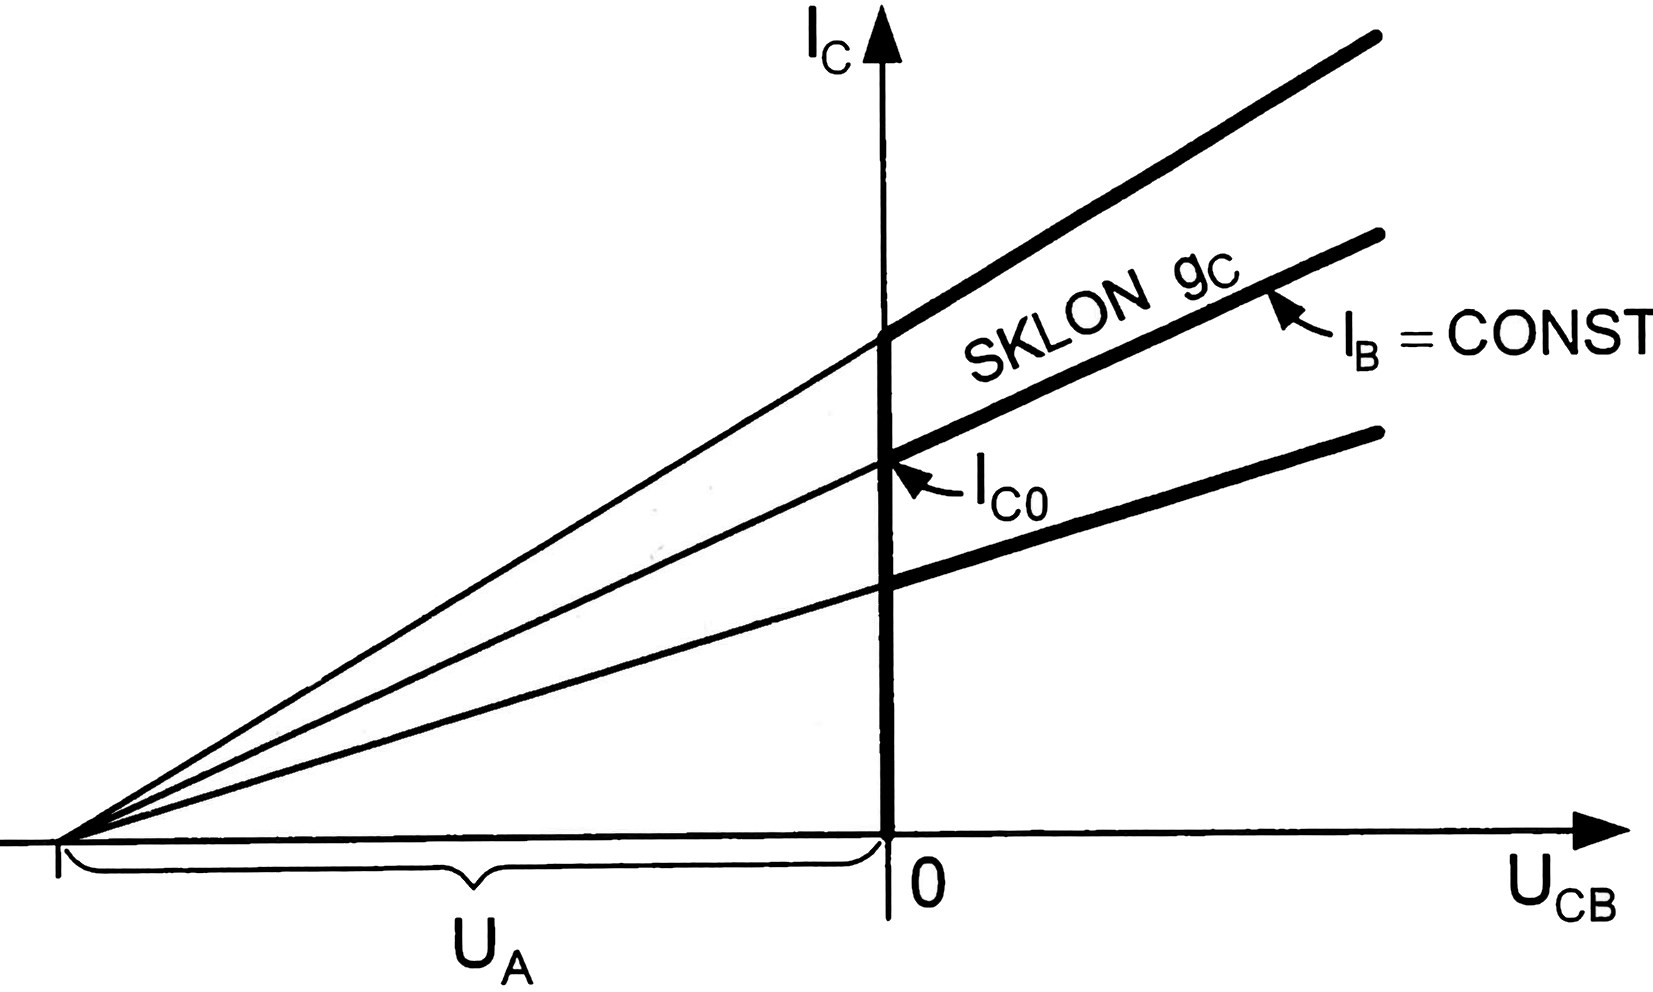
\includegraphics[width=0.6\linewidth]{aes_fig065.jpg}
          \caption{Interpretace Earlyho napětí \(U_A\) v kolektorových charakteristikách
                   \(I_C(U_{CB})\). (\cite[s.~54]{Dostal})}
          \label{aes:fig065}
        \end{figure}

        Typická velikost Earlyho napětí vstupních tranzistorů operačního zesilovače je \(U_A=
        \SI{50}{\V}\). Jinak řečeno, nasycený proud \(I_S\) a proudové zesílení \(\beta\) se
        zvětšují přibližně o \SI{2}{\percent} z výchozí hodnoty \(I_{S0}\) nebo \(\beta_0\) na každý
        \SI{1}{\V} kolektorového napětí \(U_{CB}\). Výrobní rozptyl Earlyho napětí je typicky
        \SI{50}{\percent} v souboru nevybíraných tranzistorů téhož technologického typu a
        \SI{10}{\percent} až \SI{0.1}{\percent} mezi dvěma tranzistory monolitické dvojice.

    \subsection{Unipolární vstupní stupeň}\label{aesIchIIIsecIIIssecII}
    \subsection{Konstrukční úpravy vstupního stupně}\label{aesIchIIIsecIIIssecIII}
    \subsection{Výstupní stupeň}\label{aesIchIIIsecIIIssecIV}
    \subsection{frekvenční kompenzace}\label{aesIchIIIsecIIIssecV}

%---------------------------------------------------------------------------------------------------